\documentclass[USenglish,oneside,twocolumn]{article}
\usepackage{etex}

\usepackage[utf8]{inputenc}
\usepackage[big]{dgruyter_NEW}

\usepackage{mathtools}
%\usepackage{tikz}
%\usetikzlibrary{decorations.text}
%\usepackage{tkz-berge}
\usepackage{amsfonts}
%\usepackage{natbib}

%\usepackage[urlbordercolor={1 1 1},citebordercolor={1 1 1},linkbordercolor={1 1 1}]{hyperref}
\usepackage{enumitem}
\usepackage{amsmath}
\usepackage{tabularx}
\usepackage{graphicx}
\usepackage{epstopdf}
\usepackage{titlesec}
\usepackage{upgreek}

%\titleformat{\section}
%{\normalfont\Large\bfseries}{\thesection}{1em}{}
%\titleformat{\subsection}`
%{\normalfont\large\bfseries}{\thesubsection}{1em}{}
%\titleformat{\subsubsection}
%{\normalfont\normalsize\bfseries}{\thesubsubsection}{1em}{}

\titlespacing{\section}{0pt}{15pt}{10pt}
\titlespacing{\subsection}{0pt}{10pt}{5pt}
\titlespacing{\subsubsection}{0pt}{5pt}{1pt}
 \titleformat*{\section}{\Large\raggedright\sffamily\selectfont\bfseries\mathversion{bold}}
 

\cclogo{
\includegraphics{by-nc-nd.pdf}}

% https://tex.stackexchange.com/questions/42271/floor-and-ceiling-functions
\DeclarePairedDelimiter{\ceil}{\lceil}{\rceil}
\DeclarePairedDelimiter{\floor}{\lfloor}{\rfloor}

\newcommand*\concat{\mathbin{\|}}
\newcommand*\nWinners{\left\vert{W_{i}}\right\vert}

% http://www.tapdancinggoats.com/easy-scientific-notation-in-latex.htm
\providecommand{\e}[1]{\ensuremath{\times 10^{#1}}}

\newcolumntype{L}[1]{>{\hsize=#1\hsize\raggedright\arraybackslash}X}%
\newcolumntype{R}[1]{>{\hsize=#1\hsize\raggedleft\arraybackslash}X}%
\newcolumntype{C}[2]{>{\hsize=#1\hsize\centering\arraybackslash}X}%
  
\begin{document}

\title{\huge The Onion Name System \large \\ Tor-powered Decentralized DNS for Tor Onion Services}
%\subtitle{Tor-powered Decentralized DNS for Tor Hidden Services}
\runningtitle{The Onion Name System -- Tor-powered Decentralized DNS for Tor Onion Services}

%\author[1]{Anonymized Submission}
\author[1]{Jesse Victors}
\author[2]{Ming Li}
\author[3]{Xinwen Fu}
\affil[1]{Cigital, Inc. \newline \hspace{2em} E-mail: kernelcorn@torproject.org}
\affil[2]{Department of Electrical and Computer Engineering, University of Arizona, Tucson, AZ \newline \hspace{2em} E-mail: lim@email.arizona.edu}
\affil[3]{Department of Computer Science, University of Massachusetts Lowell, Lowell, MA \newline \hspace{2em} E-mail: xinwenfu@cs.uml.edu}

% OnioNS resists Sybil attacks and computationally-powerful adversaries. 
\begin{abstract} {
Tor onion services, also known as hidden services, are anonymous servers of unknown location and ownership that can be accessed through any Tor-enabled client. They have gained popularity over the years, but since their introduction in 2002 still suffer from major usability challenges primarily due to their cryptographically-generated non-memorable addresses. \newline \hspace*{1em} In response to this difficulty, in this work we introduce the Onion Name System (OnioNS), a privacy-enhanced decentralized name resolution service. OnioNS allows Tor users to reference an onion service by a meaningful globally-unique verifiable domain name chosen by the onion service administrator. We construct OnioNS as an optional backwards-compatible plugin for Tor, simplify our design and threat model by embedding OnioNS within the Tor network, and provide mechanisms for authenticated denial-of-existence with minimal networking costs. We introduce a lottery-like system to reduce the threat of land rushes and domain squatting. Finally, we provide a security analysis, integrate our software with the Tor Browser, and conduct performance tests of our prototype.
}
\end{abstract}
  
%\keywords{Tor, DNS, name resolution, privacy} %todo?
%\classification[PACS]{}
%\communicated{...}
%\dedication{...}

%todo
\journalname{Proceedings on Privacy Enhancing Technologies}
%\DOI{Editor to enter DOI}`
%\startpage{1}
\received{2015-11-30}
\revised{2016-06-14, 2016-08-29}
\accepted{2016-08-30}

\journalyear{2017}
\journalvolume{2017}
\journalissue{1}
 
\maketitle

\vspace{-30px}

\section{Introduction}

%As the prevalence of the Internet and other communication has grown, so too has the development and usage of privacy-enhancing systems. These are protocols that provide privacy by obfuscating the link between a user's identity or location and their communications. Following a general distrust of unsecured Internet communications and in light of the 2013-current revelations by Edward Snowden of international Internet mass-surveillance, users have increasingly turned to these tools for their own protection.
%\newpage
Tor \cite{dingledine2004tor} is a third-generation onion routing system and is the most popular low-latency anonymous communication network in use today. In Tor, clients construct a layered encrypted communications circuit over three onion routers in order to mask their identity and location. As messages travel through the circuit, each onion router in turn decrypts their encryption layer, exposing their respective routing information. The first router is only exposed to the client's IP address while the last router conducts Internet activities on the user's behalf. This provides end-to-end communication confidentiality of the sender. %Tor has grown in popularity since Edward Snowden's 2013 revelations of international Internet mass-surveillance.

%The Tor network is managed by set of nine directory authorities, spread out across geographically diverse locations. Once per hour, the directory authorities vote on the state of the network and redistribute routing information to all relays and clients, forming a PKI and a information

Tor users interact with the Internet and other systems over Tor via the Tor Browser, a security-enhanced fork of Firefox ESR. This achieves a level of usability but also security: Tor achieves most of its application-level sanitization via privacy filters in the Tor Browser. Unlike its predecessors, Tor performs little sanitization itself. Tor's threat model assumes that the capabilities of adversaries are limited to traffic analysis attacks on a restricted scale; they may observe or manipulate portions of Tor traffic, that they may run onion routers themselves, and that they may compromise a fraction of other existing routers. Tor's design centers around usability and defends against these types of attacks.

\subsection{Motivation}

Tor also supports \emph{onion services} -- anonymous servers that intentionally mask their IP address through Tor circuits. They utilize the .onion pseudo-TLD, typically preventing the services from being accessed outside the context of Tor. Onion services are only known by their public RSA key and typically referenced by their address, 16 base32-encoded characters derived from the SHA-1 hash of the server's key, i.e. \url{3g2upl4pq6kufc4m.onion}. This builds a publicly-confirmable one-to-one relationship between the public key and its address and allows onion services to be accessed via the Tor Browser by their onion address within a distributed environment. Fig. \ref{fig:OnionCommunication} illustrates how clients communicate with onion services.

\begin{figure}[t!] % htbp
	\centering
	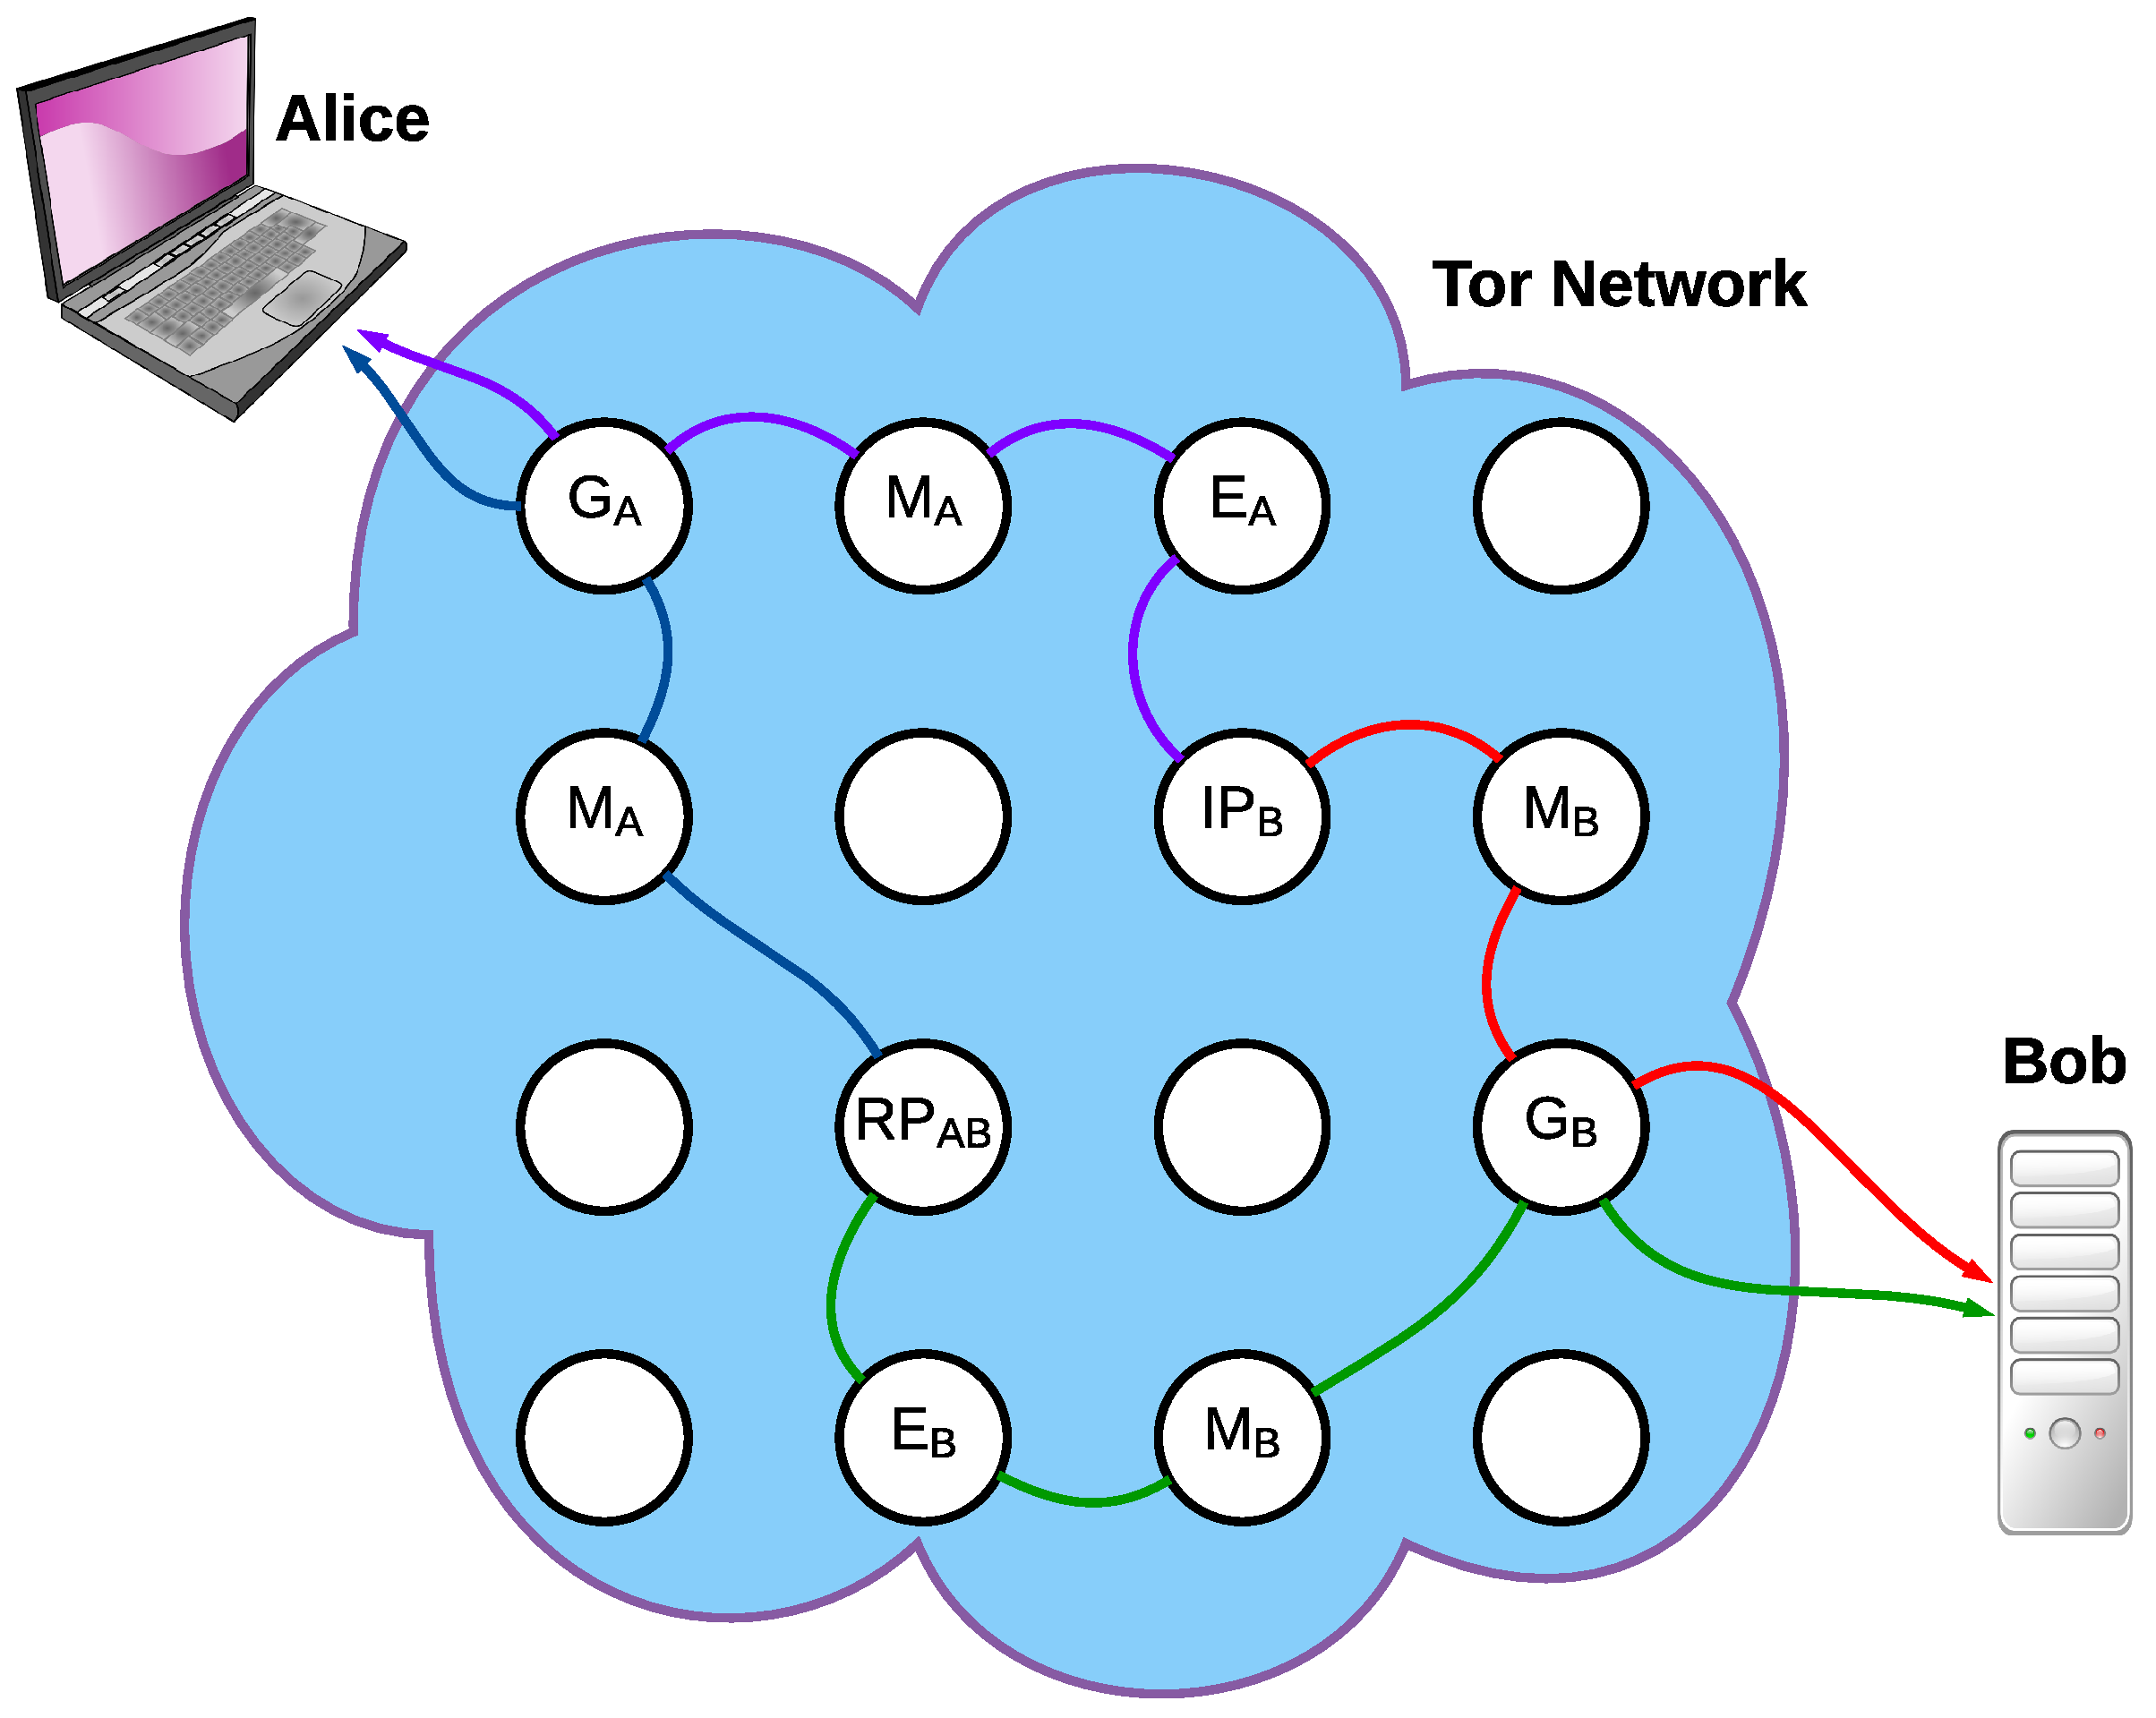
\includegraphics[width=0.8\linewidth]{../assets/images/LucidCharts/Hidden_Services.pdf}
	\caption{A Tor client, Alice, and an onion service, Bob, first mate two Tor circuits (purple and red) at one of Bob's long-term \emph{introduction points} (IP). They then renegotiate and communicate over another pair of Tor circuits (blue and green) at an ephemeral \emph{rendezvous point} (RP). This achieves communication with bi-directional anonymity \cite{overlier2006locating}.}
	\label{fig:OnionCommunication}
	
	\hspace{5px}
	
	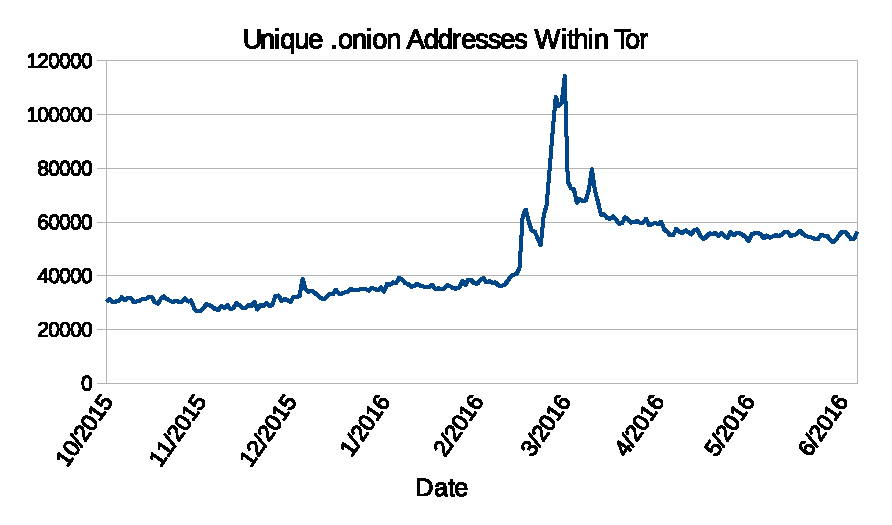
\includegraphics[width=0.85\linewidth]{../assets/images/Tor/unique_addresses.eps}
	\caption{The number of unique onion addresses seen in the Tor network between October 2015 and June 2016. \cite{TorMetrics}.}
	\label{fig:OnionCount}
	\vspace{-3px}
	
\end{figure}

Tor onion addresses are decentralized and globally collision-free, but there is a strong discontinuity between the address and the service's purpose. As their addresses usually contain no human-readable information, a visitor cannot categorize, label, or authenticate onion services in advance. While a Tor user may explore and bookmark onionsites within the Tor Browser, this is a very narrow solution and does not scale well past a few dozen bookmarks. Over time, third-party directories -- both on the clearnet and onionspace -- have appeared in an attempt to counteract this issue, but these directories must be constantly maintained and the approach is neither convenient nor does it practically scale past several hundred entries. The approximately 55,000 onion services currently on the Tor network (Fig. \ref{fig:OnionCount}) and the potential for continued growth both suggest the strong need for a more complete and wider solution to solve the usability issue.

\subsection{Contributions}

In this paper, we present the design, analysis, and implementation of the Onion Name System  (OnioNS), a decentralized, secure, and usable domain name system for Tor onion services. Any onion service administrator can claim a meaningful human-readable domain name without loss of anonymity and clients can query against OnioNS in a privacy-enhanced and verifiable manner. OnioNS is powered by a random subset of Quorum nodes within the existing Tor network, significantly limiting the additional attack surface. We devise a distributed database that is resistant to node compromise and provides proofs for authenticated denial-of-existence. We also design a novel lottery-based domain registration protocol to mitigate of denial-of-registration attacks and analyzed its security. We provide a backwards-compatible plugin for the Tor Browser and demonstrate the low latency and high performance of OnioNS. To the best of our knowledge, this is the first alternative DNS for Tor onion services which is decentralized, secure, and privacy-enhanced. %Moreover, no other alternative DNS provides mechanisms for authenticated denial-of-existence.

\textbf{Paper Organization:} This paper is divided into eight main sections. In Section \ref{sec:problemStatement} we define our design objectives and explain why existing works do not meet our goals. In Section \ref{sec:RelatedWorks} we list prominent existing works. In Section \ref{sec:threatModel}, we define our threat model, which includes Tor's assumptions and the capabilities of our adversaries. In Section \ref{sec:Solution}, we describe the system overview and define several key protocols. In Section \ref{sec:Analysis} we analyze the security of our assumptions and examine other attack vectors. In Section \ref{sec:Evaluation} we describe and demonstrate our implementation prototype and carry out performance analysis tests. Section \ref{sec:Discussions} contains further comparisons with related works. We conclude in Section \ref{sec:Conclusion}.

\section{Problem Statement}
\label{sec:problemStatement}

To integrate with Tor, we must provide a secure system, preserve user privacy, and avoid compromising other areas of the Tor network. Additionally, we seek to construct a distributed system and to providing a mechanism for authenticated denial-of-existence, which we describe in Section \ref{sec:authDenial}.

\subsection{Design Objectives}

Tor's privacy-enhanced environment introduces distinct challenges to any new infrastructure. Here we enumerate a list of requirements that must be met by any naming system applicable to Tor onion services. In Section \ref{sec:RelatedWorks} we analyze existing works and show how these systems do not meet these goals and in Section \ref{sec:Solution} we demonstrate how we overcome them with OnioNS.

1. \textbf{Anonymous registrations}: The system should not require any personally-identifiable or location information from the registrant. Tor onion services publicize no more information than a public key and a set of Introduction Points.

2. \textbf{Privacy-enhanced queries}: Clients should be anonymous, indistinguishable, and unable to be tracked by name servers. Tor already tunnels most Internet DNS queries over circuits, thus any alternative naming system should continue to preserve user privacy during lookups.

3. \textbf{Strong integrity}: Clients must be able to verify the authenticity of a domain-address pairing with cryptographic guarantees. This objective provides a defense against phishing attacks from malicious name servers.

4. \textbf{Globally unique domain names}: Any domain name of global scope must point to at most one server.  Unique domain names prevent fragmentation of users and also provides a defense against phishing attacks.

%For naming systems that generate names via cryptographic hashes, the key-space must be of sufficient length to resist cryptanalytic attack.

5. \textbf{Decentralized control}: Central authorities carry absolute control over the system and root security breaches can easily compromise the integrity of the entire system. They may also be able to compromise the privacy of both users and onion services or may not allow anonymous registrations.

6. \textbf{Low latency}: The Tor network introduces noticeable latency into communication, especially for onion services, although this is not by design. The system must promptly resolve queries to avoid negatively impacting usability and exhausting the patience of Tor users.

7. \textbf{Optional}: Not all onion services require meaningful names. For example, applications such as Ricochet \cite{RicochetGithub} may create ephemeral onion services where names may not be appropriate or necessary. Thus a naming system should be optional but not required. Systems that provide backwards compatibility by preserving the Tor onion service protocol also achieve this property.

8. \textbf{Lightweight}: In most realistic environments clients have neither the bandwidth nor storage capacity to hold the system's entire database, nor the capability of meeting significant computation burdens. The system should have a minimal impact on Tor clients and onion services.

\vspace{-10pt}
\section{Related Works}
\label{sec:RelatedWorks}

Vanity key generators (e.g. Shallot \cite{KatmagicShallot}) attempt to find by brute-force an RSA key that generates a partially-desirable hash. Vanity key generators are commonly used by onion service administrators to improve the recognition of their onion service, particularly for higher-profile services. For example, an onion service administrator may wish to start his service's address with a meaningful noun so that others may more easily recognize it. However, these generators are only partially successful at enhancing readability because the size of the domain key-space is too large to be fully brute-forced in any reasonable length of time. If the address key-space was reduced to allow a full brute-force, the system would fail to be guaranteed collision-free. Nicolussi suggested changing the address encoding to a delimited series of words, using a dictionary known in advance by all parties \cite{nicolussi2011human}. While Nicolussi's encoding improves the readability of an address, like vanity key generators it does not allow addresses to be completely meaningful.

The Internet DNS is already well established as a fundamental abstraction layer for Internet routing. However, despite its widespread use, DNS suffers from several significant shortcomings and fundamental security issues that make it inappropriate for use by Tor onion services. First, the Internet DNS does not use any cryptographic primitives. DNSSEC is primarily designed to prevent forgeries and DNS cache poisoning from intermediary name servers and it does not provide any degree of query privacy \cite{wachs2014censorship}. Additional protocols such as DNSCurve \cite{bernstein2009dnscurve} have been proposed, but DNSCurve has not yet seen widespread deployment across the Internet. Secondly, both DNS and DNSSEC are highly centralized; the entire .com TLD, for example, is under the control of Verisign in the USA. The lack of default security in DNS and its fundamental centralization prevent us from using it for onion services.

OnionDNS \cite{scaife2015oniondns} is a seizure-resistant alternative resolution service for the Internet. OnionDNS is based on DNS and uses unmodified BIND client software but anonymizes the root server by hosting it as an onion service. While OnionDNS does not require the user to install specialized software and it provides DNSSEC and other authentication mechanisms, the system is centralized by a single root server and thus  vulnerable if the root is malicious or is compromised. Although there is a separation of duties in OnionDNS to allow for revocation should the main signing key be compromised, the revocation could take a long time.  In contrast, our scheme is decentralized. In addition, in OnioNS we propose a lottery-based domain registration protocol, which effectively mitigates denial-of-registration attacks even when the attacker compromises and colludes with some Quorum nodes and has partial information about other registrants. Note that OnionDNS and OnioNS were named independently and readers should take care to not confuse the two works.

The GNU Name System \cite{wachs2014censorship} (GNS) is a decentralized alternative DNS. GNS distributes names across a hierarchical system of zones constructed into directed graphs. Each user manages their own zone and distributes zone access peer-to-peer within social circles. However, GNS does not guarantee that names are \emph{globally} unique. Furthermore, the selection of a trustworthy zone to use would be a significant challenge for using GNS for Tor onion services and such a selection centralizes control of the system. Awerbuch and Scheideler constructed a decentralized peer-to-peer naming system \cite{awerbuch2004group}, but like GNS, made no guarantee that domain names would be globally unique.

Namecoin \cite{NamecoinHome} is an early fork of Bitcoin \cite{nakamoto2008bitcoin} and is the first fully-distributed alternative DNS that distributes meaningful and unique names. Like Bitcoin, Namecoin holds information transactions in a decentralized ledger known as a blockchain. Transactions and information are added to the head of the blockchain by ``miners,'' who solve a proof-of-work problem to generate the next block. Users may also register DNS records or other information, which consumes Namecoins. While Namecoin is often advertised as capable of assigning names to Tor onion services, it has several practical issues that make it generally infeasible to be used for that purpose. First, Namecoin generally requires clients to pre-fetch the blockchain which introduces significant logistical issues due to high bandwidth, storage, and CPU load. Second, since the blockchain is an append-only data structure, it becomes less practical over time and scales poorly to high levels of activity and popularity. Third, although Namecoin supports anonymous ownership of information, it is non-trivial to anonymously purchase Namecoins, thus preventing domain registration from being privacy-enhanced. These issues prevent Namecoin from being a practical alternative DNS for Tor onion services. 

% todo: explain why the SPV or whatever clients don't work, or include OnionDNS's criticisms. This might not be necessary.
\vspace{-10pt}
\section{Assumptions and Threat Model}
\label{sec:threatModel}

We assume that Tor circuits provides privacy and anonymity. If Alice constructs a three-hop Tor circuit to Bob with modern Tor cryptographic protocols and sends a message $ m $ to Bob, we assume that Bob can learn no more about Alice than the contents of $ m $. This implies that if $ m $ does not contain identifiable information, Alice is anonymous from Bob's perspective. This also implies an assumption on the security of cryptographic primitives and a lack of backdoors or analogous breaks in cryptographic libraries. The security of Tor circuits is also dependent on the assignment of consensus weight. We assume that the majority of directory authorities are at least semi-honest so that consensus weight is an effective defense against Sybil attacks. We also assume that honest parties control the majority of Bitcoin's computational power, which implies that the Bitcoin blockchain is secure. We note that these assumptions are already made by Bitcoin and Tor and have held over time.

We assume that an active attacker, Mallory, controls some percentage of dishonest colluding Tor routers as well as semi-honest routers; however this percentage is small enough to avoid violating our previous assumption. We assume a fixed percentage of dishonest and semi-honest routers; namely that the percentage of routers under Mallory's control does not increase in response to the inclusion of OnionNS into Tor infrastructure. This assumption simplifies our threat model analysis but we consider it realistic because while Tor traffic is purposely secret as it travels through the network, we consider OnioNS information public so we don't consider the inclusion of OnioNS a motivating factor to Mallory. However, we allow Mallory to operate and actively MitM attack any of our non-authoritative name servers.

% Let $ R $ be a set of Tor routers with the Fast, Stable, and Running flags and let $ \mathit{qc} \in R $ be the set of agreeing routers with the largest cumulative amount of consensus weight. If an $ M $-sized set $ Q $ is randomly chosen from $ \mathit{qc} $ with selection probability determined by the consensus weight of each member in $ \mathit{qc} $, then we assume that the largest subset of agreeing routers in $ Q $ are at least semi-honest.

% Finally, we assume that all participants in our system -- innocent onion services as well as adversaries -- operate under some fixed budget, namely that they have an economical or time quota on the memory and CPU resources that they can allocate against our system. We also assume that an adversary may run operate any of the non-authoritative name servers.

% We further assume that an adversary may try to gain control of authoritative OnioNS servers through a Sybil attack on the Tor network or that they may 

As onion services require no more than a configured Tor client and a socket listener and are thus cheap to create, we anticipate that actors in our system will perform any of the following use cases:

\begin{enumerate}
	\item Create many onion services and attempt to register many names.
	\item Create one onion service and attempt to register many names.
	\item Create many onion services and attempt to register a single name.
	\item Create one onion service and attempt to register a single name.
\end{enumerate}

Scenarios one and two are expected to be performed by adversaries attempting to register all popular names in a ``land rush'' for financial gain or as a denial-of-registration attack. Scenario three may indicate an attempt by many legitimate actors  to claim a highly desirable name, while scenario four is the expected behavior of innocent actors. As onion services are anonymous by nature, it is impossible to construct a system that differentiates and selects between a single actor performing the first scenario and many actors performing the fourth scenario. However, we expect innocent actors to follow the fourth use case such that one entity (considering load-balancing) hosts one onion service.

% as well-known onion services cannot change their public key, 

\vspace{-5pt}

\section{Design of OnioNS}
\label{sec:Solution}
\vspace{-5pt}
\subsection{Cryptographic Primitives}
\label{sec:cryptoPrimitives}
\vspace{-5pt}

OnioNS utilizes hash functions, digital signature algorithms, a proof-of-work scheme, and a global source of randomness.

\begin{itemize}
	\item $ \mathcal{H}(x) $ is a cryptographic hash function of a message $ x $. We define $ \mathcal{H}(x) $ as SHA-256.
	\item $ S_{\mathit{RSA}}(m, r) $ is a RSA digital signature function that accepts a message $ m $ and a private RSA key $ r $ and returns a digital signature. Let $ S_{\mathit{RSA}}(m, r) $ use $ \mathcal{H}(x) $ as a digest function on $ m $ in all use cases. We define $ S_{\mathit{RSA}}(m, r) $ as EMSA4/EMSA-PSS.
	\item $ V_{\mathit{RSA}}(m, S, R) $ validates an RSA digital signature by accepting a message $ m $, a signature $ S $, and a public key $ R $, and return true if and only if the signature is valid.
	\item $ \mathrm{PoW}(x) $ is a one-way function that accepts an input key $ k $ and returns a deterministic output. While $ \mathrm{PoW}(x) $ could ideally be set to memory-hard key derivation function such as scrypt \cite{percival2012scrypt}, for performance reasons we define $ \mathrm{PoW}(x) $ as $ \mathcal{H}(x) $.
	\item $ \mathcal{G}(t) $ is a cryptographically-secure beacon of random numbers. $ \mathcal{G}(t) $ periodically returns a random number at time $ t $, which is unpredictable before $t$ but is publicly verifiable after $t$. %As explained in Section \ref{sec:rngProcess}, we derive $ \mathcal{G}(t) $ from Bitcoin.
	\item $ \mathcal{R}(s) $ is a cryptographically-secure pseudorandom number generator (CSPRNG) that accepts an initial seed $ s $ and returns a list of pseudorandom numbers. In our design, $ s = \mathcal{G}(t) $. For efficiency reasons, we suggest AES in CTR mode using $ s $ as a key with a fixed IV.
\end{itemize}

\subsection{Definitions}

This section lists commonly-used terms and Table 1 defines frequent mathematical notation.

The syntax of OnioNS \textbf{domain names} mirrors the Internet DNS; we use a sequence of name-delimiter pairs with a .tor pseudo-TLD. The Internet DNS defines a hierarchy of administrative realms that are closely tied to the depth of each name. By contrast, OnioNS makes no such distinction. We let onion service administrators claim second-level names and then control all names of greater depth under that second-level name.

A \textbf{ticket} is a small and fundamental data structure. It contains $ \mathit{type} $, $ \mathit{name} $, $ \mathit{secondaryAddrs} $, $ \mathit{subdomains} $, $ \mathit{contact} $, $ \mathit{rand} $, $ \mathit{signature} $, and $ \mathit{pubHSKey} $. Tickets by default have $ \mathit{type} $ set to ``ticket'', but this data structure becomes a \textbf{record} if $ \mathit{type} $ is set to any of the operations described in Section \ref{sec:recordOps}.

A \textbf{mirror} is Tor router that is acting as a name server within the OnioNS network. Mirrors maintain a textual database of system information and respond to client queries but usually do not accept new DNS records or other information from onion services. We note that mirrors may be outside the Tor network, but this scenario is outside the scope of this work.

\textbf{Quorum candidates} are mirrors that hold a current copy of the database. They also have sufficient CPU and bandwidth capabilities to handle OnioNS communication in addition to their normal Tor duties.

The \textbf{Quorum} is an authoritative subset of Quorum candidates who have active responsibility to maintain the OnioNS database. Quorum nodes accept and process information from onion services but do not respond to client queries. The Quorum is randomly chosen from the set of Quorum candidates and is rotated periodically, as described in Section \ref{sec:protocols}.

\begin{center}
	\vspace{-5mm}
	\begin{table}[htp]
		\centering
  		\begin{tabular}{ | c | l | }
			$ \left\vert{S}\right\vert $ & the cardinality of the set $ S $ \\ \hline
			$ \left\vert{T}\right\vert $ & number of routers in the Tor network \\ \hline
			$ \left\vert{Q}\right\vert $ & size of the Quorum \\ \hline
			$ Q_{i} $ & the $ i $th Quorum where $ i $ is an iteration counter \\ \hline
			$ \Delta q $ & lifetime of the Quorum \\ \hline
			$ r(f) $ & if $ r $ is a record, the field $ f $ in $ r $ \\
		\end{tabular}
		\caption{Frequently used notations.}
	\end{table}
	\vspace{-45pt}
	\label{table:freqUsedNotation}
\end{center}

\subsection{Infrastructure}

We embed OnioNS infrastructure within the Tor network by utilizing existing Tor nodes as hosts for OnioNS mirrors. Each Tor node may opt to run an onion service which then powers an OnioNS mirror server running on localhost. As these onion services are part of OnioNS, they must be accessed by their traditional .onion address, but this is acceptable as these servers are never accessed directly by end-users. Our reliance on onion services allows us to reuse existing TLS links between Tor nodes and leverage Tor circuits to obscure all communication between end-users and OnioNS infrastructure without requiring a modification to the Tor executable. In essence, all communication with or within OnioNS is hidden from outside observers by ephemeral internal Tor circuits, increasing privacy and reducing our attack surface. %  that need not pass through exit routers

We authenticate servers in our infrastructure using Ed25519 \cite{bernstein2012high} keys. Starting with Tor 0.2.7, Tor routers generate and manage Ed25519 keypairs and include their public key in the network consensus. We use Ed25519 because of its strength, size, and speed advantages over Tor's original RSA-1024 identity keys. OnioNS servers use their private key to digitally sign outbound traffic from their onion service, achieving end-to-end authentication of all OnioNS communication.
% Throughout the remainder of this paper, ``onion services'' refers exclusively to onion services that are not part of the OnioNS infrastructure.

\subsection{Overview}
\label{sec:overview}

The data flow in OnioNS is illustrated in Fig. \ref{fig:dataFlow}. First, all parties retrieve $ \mathcal{G}(t) $ (a beacon) from the Bitcoin network, shown via a blue dash line. They then use CSPRNG $ \mathcal{R}(\mathcal{G}(t)) $ to select a set of Quorum nodes (Q) within the Tor network. Second, an onion service (OS) sends tickets or records to the Quorum. Since mirrors (M) subscribe to Quorum nodes, this data also propagates to mirror nodes. Each mirror maintains a Merkle tree of all the records obtained from the Quorum. At a later point, a client can query the mirror for the record. The mirror returns the ticket or record along with a path through the Merkle tree, shown in solid black. The client then verifies the Merkle tree proof and checks that the majority of Quorum published the same root in the network consensus document (CD), shown in the purple dash-dotted line. This procedure occurs much the same way even if no such ticket or record exists for a given name. %Thus, OnioNS relies on the majority of Quorum to be honest.

\begin{figure}[t!] % t!
	\centering
	
	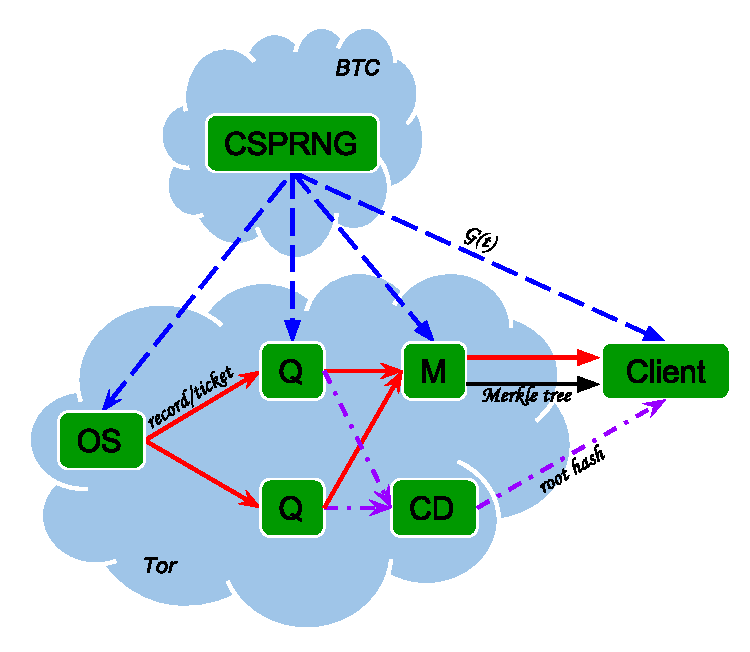
\includegraphics[width=0.88\linewidth]{../assets/images/protocol_overview.eps}
	\caption{An overview of data flow in OnioNS. }
	\label{fig:dataFlow}
	
	\hspace{0px}
	\vspace{-10pt}	
	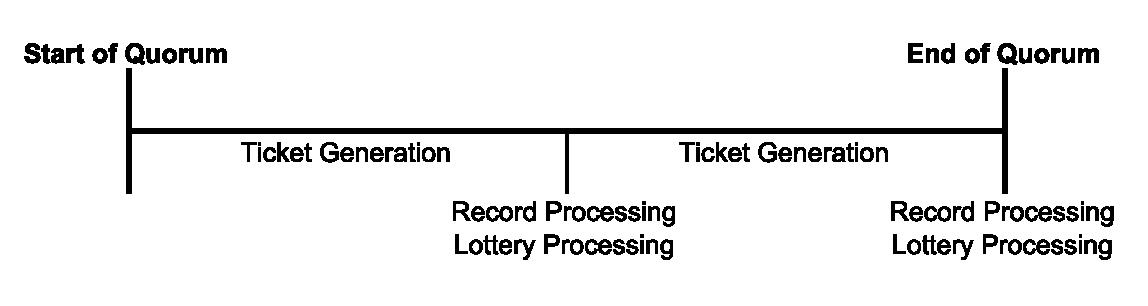
\includegraphics[width=\linewidth]{../assets/images/quorum_timeline.eps}
	\caption{The series of events within each Quorum's lifetime. }
	\label{fig:quorumTimeline}
	\vspace{-7pt}
\end{figure}

Next, we explain the series of events within each Quorum's lifetime. A set of Quorum nodes' lifetime can span one or multiple registration periods, each being 24 hours long, wherein onion services apply for a meaningful name by generating a ticket and performing proof-of-work. At the end of each registration period, Quorum nodes process the tickets received during that period, and use a new value of $ \mathcal{G}(t) $ to determine a subset of registrants that have won the lottery. These onion services then receive their meaningful name and their records are added to the Quorum's and mirrors' name databases. This cyclic process is illustrated in Fig. \ref{fig:quorumTimeline}.

%Mirrors return records from this database to clients, who can then use the published state to authenticate the mirror's responses, as described in Section \ref{sec:authDenial}. 
% Twelve hours prior to the rotation of the Quorum, mirrors merge the ephemeral database into the authenticated database and publish the new state of the authenticated database in the network consensus, as described in Section \ref{sec:qQualification}.

%nuance: repeated information is not replayed
% some Q members could be malicious, how are subscriptions handled?

\subsection{Protocols}
\label{sec:protocols}

We now describe the protocols fundamental to OnioNS functionality. These protocols are listed according to their approximate order of execution in OnioNS.

\subsubsection{Random Number Generation}
\label{sec:rngProcess}

$ \mathcal{G}(t) $ is used as a basis for several of our protocols. The key issue is how to obtain a secure and decentralized source of randomness.  One straightforward definition of $ \mathcal{G}(t) $ is the SHA-256 hash of Tor's consensus documents. If the Tor network is dynamic enough to provide significant amounts of entropy into the consensus documents, then $ \mathcal{G}(t) $ may be considered cryptographically secure. However, this assumption does not hold because current router descriptors are publicly available before the consensus documents are published, allowing $ \mathcal{G}(t) $ under this approach to be easily manipulated by a few malicious Tor routers. The attack becomes significantly easier in the final moments before the directory authorities publish the consensus.

Another alternative approach is the commitment scheme proposed by Goulet and Kadianakis \cite{GouletCommitReveal}. Their algorithm modifies the consensus voting protocol that is run once an hour by Tor directory authorities. In their scheme, at 00:00 UTC each authority commits a SHA-256 hash of a secret value $ v $ into each consensus vote across a 12 hour period. Then at 12:00 UTC, each directory authority reveals $ v $ across the next set of 12 consensuses. Finally, at 24:00 UTC, the revealed values are hashed together to create a single random number, which is then embedded in the consensus documents so that it is efficiently distributed to both Tor routers and clients. A different random number thus appears in the consensus every 24 hours. 

However, the above commitment scheme has a well-known weakness when some of the directory authorities are malicious. Namely, while reveals must demonstrably match commits, each participant may choose to reveal or not. If they do not reveal, their value is lost and the protocol produces a different output. If Mallory controls $ b $ participants, she can make this choice with each participant in turn, allowing $ 2^{b} $ different outcomes, which can be used for Mallory's favor, e.g. skew the RNG output to select malicious and colluding Quorum nodes. Since preventing such attack requires trust in all nine directory authorities, which is contradictory to our goal of decentralization, we will not use this approach.

Instead, we propose to construct $ \mathcal{G}(t) $ using the latest block in the longest (and most secure) Bitcoin blockchain. Bitcoin blocks consist of an 80-byte header and an array of transactions. The block header contains a version number, timestamp, current difficulty level $d$, a 32-bit nonce, a SHA-256 hash of the previous block header, and a SHA-256 root hash of the Merkle tree constructed from all transactions in that block. Among these items, the nonce and Merkle hash are the main contributors of entropy for the block header, since the rest are predictable given all the previous blocks. According to the recent analysis by Bonneau, Clark, and Goldfeder \cite{BonneauCG15}, the amount of (computational) min-entropy contained by a block header is $ d $ bits, (currently $ d > 68 $) from which one can extract a near-uniform random number of at least 32 bits long. Since the blockchain's security relies on the assumption that honest parties control the majority amount of computation power, the head of blockchain can be regarded as a  decentralized random source. We present more detailed analysis of security on this topic in Sec. 6.

Following the suggestion by \cite{BonneauCG15}, we construct a random beacon from the head of the blockchain as follows:  

\begin{equation}
\mathcal{G}(t) = \mathsf{Ext}_k(B_t||\mathcal{H}(B_t)),
\end{equation}

\noindent where $B_t$ is the header of the latest mined block (at time $t$) from the longest chain in Bitcoin, and $\mathit{Ext}_k$ is a standard randomness extractor such as HMAC, with $k$ as a key to randomly choose the extractor function. In Bitcoin, such a valid block is mined about every 10 minutes by design.

Tor clients and Tor routers can acquire or calculate $ \mathcal{G}(t) $  in several ways. First, they can download the entire Bitcoin blockchain from the Bitcoin network, find the block at time $ t $, and generate $ \mathcal{G}(t) $ from its header. However, this approach trades high security for significant storage, bandwidth, and processing costs, which may be impractical or prohibitive in many cases. The second method is for clients to query a trusted source for an initial ``seed block'' on the main blockchain and then download the remainder of the blockchain from that block. They can either download the blockchain peer-to-peer, from the Bitcoin network, or from a centralized server, but this choice does not matter since the chain is verified against the seed block. Periodically, clients could then reset the seed block to the latest block and repeat the process. This offers a significant reduction in overhead, but requires a trusted source for the initial seed block. The third, least secure, but cheapest method is to download the header from a trusted source. We allow Tor clients and Tor routers to perform any of these methods. We provide an onion service server for the seed block and header and note that we could also distribute $ \mathcal{G}(t) $ through the consensus documents.

%While this implementation of $ \mathcal{G}(t) $ defines $ t $ as an integer of 24 hours, $ \Delta q $ may be greater than 24 hours, as discussed in \ref{sec:qRotation}. Therefore, throughout the remainder of this document we will use the notation $ \mathcal{G}(i) $ to reference the $ \mathcal{G}(t \cdot 24 \cdot \Delta q) $ that defines $ Q_{i} $.

%JV_TODO: The publication of $ \mathcal{G}(i) $ at midnight defines the selection of the next Quorum, causes all mirrors to publish the state of their database, marks the beginning of the next domain registration game (auction and lottery), and determines the winners of the lottery?. 

% \underline{Jesse: this is not clear. The auction and lottery's time span may not be 24 hours and depends on our parameter selection like threshold difficulty. So we will need a new random number at the time when we want to do the lottery. So RNG seed is not just generated every midnight, but need a new one as we need it.}

%The first reveal at 12:00 UTC ends the lottery and contains the pool of Quorum candidates. We clarify our distinction of these boundaries in section \ref{sec:GlobalRand}. 

\subsubsection{Authenticated Denial-of-Existence}
\label{sec:authDenial}

We described earlier that a malicious name server may forge a response or may falsely claim non-existence of a name. These are attack vectors that remain open by naming systems that do not provide authentication mechanisms. We use a Merkle tree \cite{merkle1988digital} to defend against these attacks with minimal networking costs. This tree is a fundamental authentication mechanism for both existing and non-existing names. All mirrors, including Quorum nodes, perform this algorithm. The tree's root hash is then checked by clients during other protocols. Let Charlie be a mirror.

\begin{enumerate}
	\item Charlie fills an array list $ S $ with the $ r_{i}(\mathit{name}) \concat \mathcal{H}(r_{i}) $ for each record $ r_{i} $ received from onion services.
	\item Charlie sorts $ S $ by the $ \mathit{name} $ field.
	\item Charlie constructs a Merkle tree $ T $ from $ S $.
	\item Charlie publishes the root hash of $ T $ in the consensus as described in Section \ref{sec:qQualification}.
\end{enumerate}

We note that a sorted Merkle tree does not support dynamic record updates and must be rebuilt at each update. While other data structures exist that support proof of existence and non-existence and allow efficient updates, such as a skip list \cite{goodrich2001implementation}, these structures are significantly more complicated. We consider it sufficient to use a Merkle tree as the tree is only rebuilt once per day in $ \mathcal{O}(n \log(n)) $ time.

\subsubsection{Quorum Qualification}
\label{sec:qQualification}

Quorum candidates must prove that they are both up-to-date mirrors and that they have sufficient capabilities to handle the increased communication and processing demands from OnioNS protocols, an additional burden on top of their traditional Tor responsibilities.

The na\"{i}ve solution to demonstrating the first requirement is for all participants to simply ask mirrors for their internal database, and then compare the recency of its database against the databases from the other mirrors. However, this solution does not scale well. Tor has approximately 2.1 million daily users \cite{TorMetrics}: it is infeasible for any single node to handle queries from all of them. Instead, at 00:00 UTC each day, let each mirror apply any record operations that it received in the last 24 hours, recompute the Merkle tree, and place the root hash inside the Contact field of its router descriptor so that the hash appears in the network consensus. The Contact field is typically used to hold the email address and PGP fingerprint of the router's administrator, but our use of the Contact field allows us to distribute the hash without modifying Tor infrastructure. Mirrors can also distribute their onion service address in the same way. %These values could also be held in new descriptor fields, which we will explore after publication.

Tor provides a mechanism for demonstrating the latter requirement; Quorum candidates must have the Fast, Stable, and Running flags. Tor routers with higher CPU or bandwidth capabilities relative to their peers also receive a proportionally larger consensus weight from the directory authorities. This consensus weight in turn strongly influences router selection during circuit construction: routers with higher weights are more likely to be chosen in a circuit. This scheme also increases Tor's resistance to Sybil attacks. Thus, we can benefit from this infrastructure by selecting the Quorum from the pool of Quorum candidates by a similar mechanism.

\subsubsection{Quorum Formation}
\label{sec:qFormation}

Once OnioNS mirrors and Tor clients have $ \mathcal{G}(t) $, they can check the aforementioned qualifications to locally derive the current or any previous Quorum in $ \mathcal{O}(\left\vert{T}\right\vert) $ time locally without performing any additional network queries. Without loss of generality, let a client Alice run this algorithm at 00:00 UTC.

\begin{enumerate}
	\item Alice obtains and validates the consensus document $ C $ published at 00:00 UTC. Since consensus documents are timestamped and signed by Tor directory authorities, Alice may download the document from any source without loss of security.
	\item Alice obtains $ \mathcal{G}( t_1 ) $ where $t_1$> 00:00 UTC, i.e. the first beacon obtained after midnight, using the method from Section \ref{sec:rngProcess}.
	\item Alice constructs a list $ S $ from $ C $ of Quorum candidates that have the Fast, Stable, and Running flags.
	\item For each group $ g \in S $ that publishes an identical root hash, Alice computes $ s_{g} = \sum_{j=0}^{\left\vert{g}\right\vert} w_{g}(j) $ where $ w_{g}(j) $ is the consensus weight of Tor router $ j $ in group $ g $. The Quorum candidates, $ \mathit{qc} $, is the group with the largest value of $ s_{g} $.
	\item Alice uses $ \mathcal{R}(\mathcal{G}(t_1)) $ to select $ \min(\mathrm{size}(\mathit{qc}), \left\vert{Q}\right\vert) $ Quorum nodes from $ \mathit{qc} $ with the probability of selecting router $ x $ determined by 
	\[
			P(x) = \frac{w_{\mathit{qc}}(x)}{s_{\mathit{qc}}}
	\]
\end{enumerate}

For security purposes, Alice must apply $ \mathcal{G}(t_{1}) $ to a consensus document published at time $ t_{2} $, where $ t_{1} > t_{2} $. If $ t_{1} < t_{2} $, then an attacker who controls $ x $ Quorum candidates can maliciously influence Quorum selection after seeing the beacon by adding or removing some candidates from the consensus. We avoid this attack by retroactively applying the CSPRNG to an older consensus document.

\subsubsection{Database Selection}
% in implementation, Charlie asks for H(nonce + database), and nodes reject query or notify Charlie if they see the same nonce twice
	% the implementation can also repeat this algorithm periodically, could be used for choosing who to subscribe to

The OnioNS network propagates information in near real-time in a peer-to-peer fashion; mirrors open authenticated circuits to other mirrors and subscribe for new tickets and records. All Quorum nodes subscribe to each other, forming a complete graph, and non-Quorum mirrors subscribe to all Quorum nodes. Under this scheme, all mirrors that remain online and at least semi-honest will process the information. However, mirrors that drop offline will be out-of-date and must synchronize against the network by the following algorithm. Let Charlie be a mirror.

% todo: enough detail here?
\begin{enumerate}
	\item Charlie asks each Quorum node for the SHA-256 hash of all records that the node has received.
	\item Charlie finds the largest group, $ g $, of Quorum nodes that return the same hashes.
	\item Charlie uses delta compression to download recent records from any node in $ g $.
	%\item Charlie verifies that $ \mathcal{H}(\mathit{db}_{e}) $ and $ \mathcal{H}(\mathit{db}_{m}) $ match the $ g $'s hashes.
	\item Charlie verifies the integrity of all records and is fully synchronized if all records pass inspection.
\end{enumerate}

Quorum nodes that were temporarily offline conduct the same algorithm, but may also ask other Quorum nodes to replay new tickets so that they may process the lottery as part of the Domain Registration protocol. %Non-Quorum mirrors subscribe to Quorum nodes according to the same algorithm.

% When onion services transmit information to the Quorum, each Quorum node replays it to all subscribers. This allows all Quorum members to receive the same information even if the onion service transmits to only some Quorum nodes.


\subsubsection{Domain Registration}
\label{sec:ticketGeneration}

To prevent malicious domain registrations such as land-rushing and denial-of-registration attacks, we need to enforce some cost when an onion service administrator registers a domain name. A common way to do so in a distributed system is through proof-of-work (PoW) \cite{nakamoto2008bitcoin}. A PoW algorithm is usually a cryptographic challenge which is difficult to solve but easy to verify. In OnionDNS \cite{scaife2015oniondns}, the authors proposed an auction-based PoW mechanism in which the registrant who spent the most computing time for PoW wins a domain. It forces the registrants to focus their computing power on a small subset of domains rather than many at a time. However, it assumes that the game  has incomplete information, i.e. participants do not know who their opponents are in each game when they are bidding on a domain. If the game participant information is fully known to the registrants, then for games with no honest registrants, an attacker can always solve the puzzle at the minimum difficulty and therefore successfully register many names. This makes it inapplicable to our system because some of the Quorum nodes may be compromised and collude with powerful attackers trying to register many names. 

%To resolve the above challenge, we propose to extend the registration scheme in OnionDNS \cite{keylist} in two ways: (1) enforcing a threshold difficulty level of PoW for all the registrants as a barrier-of-entry (to filter the registrants into a set of candidates); (2) employ a lottery drawing on the candidate registrants to determine the final winners, so as to limit the rate of domain registration. The game consists of  two phases. 

To resolve the above challenge, we propose a lottery-based scheme. The key idea is two-fold: (1) require every registrant to submit a ``ticket'' and solve a PoW problem related to this ticket, where we enforce a threshold difficulty level of PoW for all the registrants as a barrier-of-entry; and (2) employ a weighted lottery drawing on the valid tickets to determine the final winners, so as to limit the rate of domain registration, where the weight is proportional to the computational effort spent by each registrant. The scheme consists of  two phases: first, ticket generation and submission, and second, a lottery.
 

%\textbf{Definitions}. A registration tuple from a registrant Bob includes the following: \underline{(Dr. Li: Others to add here)}
%\begin{enumerate}
%		\item[-]  \emph{name}: a meaningful domain name.
%		\item[-]   \emph{subdomains}: a map of domains of level three or higher and their respective destinations, which may be to either .tor or .onion domains.
%		\item[-] \emph{contact}: the Bob's PGP key fingerprint.
%		\item[-]  \emph{signature}:  output of $ S_{\mathit{RSA}}(\mathit{name} \concat \mathit{subdomains} \concat \mathit{contact}, r) $ where $ r $ is Bob's private RSA key.
%		\item[-]  \emph{pubHSKey}: Bob's RSA public key.
%	\end{enumerate} 
%
%The detailed steps are as follows:
%
%\textit{The auction phase}: One game is conducted for each claimed name. 
%\begin{enumerate}
%	\item Before 00:00 UTC of every day, all the registrants register their claimed domain names and the corresponding public key/private key pairs with the current quorum.  All the registrants that claim the same name participate in a single auction game. The following proceeds for each game.
%	\item The quorum generates a puzzle $p$, using the most recent head of the blockchain as a random source. Every registrant  receives an identical puzzle, and need to compute a solution $a$ such that:  
%	
%	\begin{equation}
%	\mathcal{H}(p||a) \& \{1\}^d = 0,
%	\end{equation}
%	
%	where $d$ is the difficulty level of the puzzle (number of zero leading bits), $\{1\}^d$	represents a $d$ bit string of all 1's and $\&$ 	is a bit-wise AND. 
%	
%	\item During a pre-defined time period $\Delta T_1$ after all registrants in one game receive the puzzle, they begin to solve for the puzzle and try for the maximum difficulty they can solve. When  $\Delta T_1$ ends, each participant records the most recent solution (if any) and the maximum difficulty level they have solved. Each of them sends the hash of the result to the quorum and broadcast to all peer registrants: $\mathcal{H}(\mathcal{H}(p||a))$ with its own signature using the private key, which commits the result and difficulty.
%	
%	\item After all registrants received all others'  commitments, they begin to reveal their answer $a$ and $d$ to the quorum and peer registrants, by which all of them can verify the validity of others' answers via two hash operations. 
%	
%	\item After all registrants revealed, the quorum does the following: for any registrant without a solution exceeding a threshold difficulty $d_{th}$, it is removed from the game; if none of the registrant solved a difficulty $d\geq  d_{th}$, this game ends with no winner; otherwise, it identifies the registrant   with the maximum difficulty level $d_{max}$ solved, and record it as the finalist $w_{i}$ for the auction of this game $i$. Ties are broken randomly.
%	 
%\end{enumerate}
%
%\textit{The lottery phase}:
%\begin{enumerate}
%	\item  From all the finalists $\{w_1, ..., w_n\}$ of all the games in the previous phase, a lottery is drawn to generate $X<n$ winners: For each finalist $w_i$, associate a weight equaling to its maximum difficulty level solved in previous phase $d_{max, i}$.  Compute a probability as $p_i=\frac{d_{max, i}}{\sum_{i=1}^n{d_{max, i}}}$. The lottery is drawn (without replacement) upon all the finalists with their corresponding probabilities, until $X$ finalists are drawn, which are declared as the final winners. The quorum accepts their domain registration and key pairs, and updates the database accordingly.
%\end{enumerate}
%
%The above protocol encourages everyone to dedicate  their maximum computing effort toward a single game. To deal with compromised quorum nodes colluding with attackers, there are two mechanisms: (1) the commit-and-reveal step is used to prevent the registrants knowing others' input before the auction starts, which enforces blind bidding when there are two or more participants in a game. (2) Even if a sybil attacker creates multiple names and participates in multiple games with only itself as participant, and it has this knowledge by colluding with a quorum node, it has to pass the threshold difficulty first in every game in order to be qualified as a finalist, and it has to work towards its maximum difficulty as possible in order to gain an statistical advantage in the lottery. Importantly, due to the commit-and-reveal, the attacker does not have the knowledge of other game finalists' difficulty levels when it commits its own difficulty level. Finally, even if an attacker happen to take over all the finalists (e.g., when  the number of legitimate registrants is small and they have little computing power), due to the rate limiting factor of lottery, it can only have limited number of registrations. On the other hand, for a legitimate registrant, it will dedicate all its computing power to a single game, so most legitimate registrants should have a good chance of making to the finalists.  (\underline{Dr. Li: need good parameter selection and experimental results on the number of hours and times to successfully register a domain}) 
% 

\textbf{Ticket Generation and Submission.}
The ticket generation period spans for a 24-hour period: from 00:00 UTC each day until 24:00 UTC $ - \delta t$, where $\delta t$ is a small time period (e.g., five minutes). Starting from 00:00 UTC, an onion service administrator (a.k.a. registrant), Bob, may enter into the OnioNS lottery by generating a ticket, containing a second-level domain name for his onion service. Then, all the registrants submit the hash commitment of their tickets during the submission time window [00:00 UTC, 24:00 UTC $ - \delta t $], and reveal their tickets after 24:00 UTC. 

%After 24:00 UTC, the Quorum verifies the validity of all the   tickets submitted, and draws a lottery to obtain the final winners. 
% and it may be further checked by mirrors and clients if his ticket win the lottery, so Bob must follow this protocol to ensure that his ticket is accepted by all parties.

Bob generates an initial ticket by defining the following fields:  
 \begin{enumerate}
 	\item[-] \emph{type}: ``ticket''.
 	\item[-]  \emph{name}: a meaningful domain name.
 	\item[-] \emph{secondaryAddrs}: a list of additional .onion destinations for load-balancing across multiple servers
 	\item[-] \emph{subdomains}, a map of domains of level three or higher and their respective destinations, which may be to either .tor or .onion domains.
 	\item[-] \emph{contact}: (optional) Bob's PGP key fingerprint.
 	\item[-] \emph{rand}: $ \mathcal{G}(i) $.
 	\item[-] \emph{nonce}: a nonce, which is a solution to the PoW problem.
 	 \item[-]  \emph{pubHSKey}: Bob's RSA public key.
 	\item[-]  \emph{signature}: output of  $ S_{\mathit{RSA}}(\mathit{type} \concat \mathit{name} \concat \mathit{secondaryAddrs} \concat \mathit{subdomains} \concat \mathit{contact} \concat \mathit{rand}\concat \emph{nonce}, r) $ where $ r $ is Bob's private RSA key.
 \end{enumerate} 
 
In the above, $\emph{nonce}$ should be a solution to the following PoW: 
 	
% 	\begin{equation}
% 	\mathcal{H}(\mathit{signature}||\emph{nonce}) \& \{1\}^{d_{bob}} = 0,
% 	\end{equation}
 	
 	\begin{equation}
 	v_{\mathit{PoW}} = \mathcal{H}(\mathit{signature}||\emph{nonce}) \leq v_{\textit{th}},
 	\end{equation}
 	
\noindent where $ v_{\textit{th}} \in \mathbb{Z} $ and $ v_{\textit{th}} < 2^{256} $. We use $ d_{\textit{th}}= \floor{log_2{(2^{256}/v_{\textit{th}})}}-1$ and $ d_{bob}= \floor{log_2{(2^{256}/v_{\mathit{PoW}})}}-1$ to denote the threshold and actual difficulty levels, respectively (i.e., number of leading zero  bits in the hash). %$\{1\}^d$	represents a $d$ bit string of all 1's and $\&$ 	is a bit-wise AND.
 
Note that Bob's tickets are valid only when $d_{Bob}$ is larger than a difficulty threshold set by Quorum nodes. Each iteration of the above PoW results in a different and one-way output because  $ S_{\mathit{RSA}}(m, r) $ is a probabilistic signature scheme. Bob must repeatedly resign and recompute $ \mathrm{PoW} $ until the formula is satisfied.  Note that this discourages Bob to outsource the PoW  computation to a powerful cloud service, since computing the signature requires possession of Bob's private key. Once the threshold difficulty is met, Bob must continue to search for an answer to the PoW such that it reflects the maximum difficulty (minimum $v_{\mathit{PoW}}$) he can obtain during the ticket generation period. No tickets are submitted during the ticket generation period in order to prevent malicious registrants from knowing the ticket information of other registrants in advance. During the submission time window (e.g., the last minute of the day), Bob finalizes the ticket corresponding to the solution to the PoW with minimum $v_{\mathit{PoW}}$ he obtained so far and generates a hash commitment of everything inside his ticket: $commit_{bob}=\mathcal{H}(\mathit{type} \concat \mathit{name} \concat \mathit{secondaryAddrs} \concat \mathit{subdomains} \concat \mathit{contact} \concat \mathit{rand}\concat \emph{nonce}\concat\emph{pubHSKey}\concat \emph{signature})$. Then he sends $commit_{bob}$   to all the Quorum nodes. No tickets that are submitted after the ticket generation period will be accepted for the current day's lottery. After all the tickets are submitted, all the registrants reveal their ticket contents to the Quorum. These reveals form an initial pool of tickets.

% so that each Quorum node can verify the integrity of the hash commitment and the record's signature. If a ticket passes the verification, then they include it in an initial pool of tickets.

% Note that, instead of directly submitting the solution $\emph{ans}$, Bob submits a hash commitment of it: $  \mathcal{H}{\emph{ans}}$ to the quorum. This prevents a malicious attacker from knowing Bob's answer and difficulty of his PoW and change its answer. 

\textbf{Ticket Processing.} Following the ticket reveals, each Quorum node $ Q_{i,k} $ inspects every ticket in the initial pool, finds the actual difficulty for the PoW in each ticket by recomputing $v_{\mathit{PoW}}=\mathcal{H}(\mathit{signature}||\emph{nonce})$, and performs the following to prune the tickets to form a lottery ticket pool:

\begin{enumerate}
	\item Rejects $ t $ if the hash of the record fields do not match any commitment hash.
	\item Rejects $ t $ if the $ t $'s PoW value is greater than the threshold, i.e. $v_{\mathit{PoW}}> v_{\textit{th}}$.
	\item Rejects $ t $ if the record's signature is invalid or if any other field is malformatted.
	\item Rejects $ t $ if $ t $'s \emph{name} is already registered.
	\item Rejects $ t $ if the onion service does not have a descriptor in Tor's distributed hash table.
	% \item Rejects $ t $ if the onion service cannot answer an HTTP GET request.
	% \item Rejects $ t $ if the response from an HTTP GET matches any other response from previous tickets.
	\item Otherwise, it records $ t $ in its lottery pool, $ T_{i} $.
\end{enumerate}

%for each domain name that is being claimed by the initial ticket pool, whenever there are multiple tickets registering the same domain name,  it compares the actual difficulty level of those tickets, and only retain the ticket with the maximum difficulty level. Ties are broken randomly, using $ \mathcal{R}(\mathcal{G}(i + 1)) $. If there is only one ticket under a name,

%The ticket generation process ends at 24:00 UTC of the same day, after which no tickets will be accepted for the day, and then the lottery phase begins. When the ticket generation phase ends, each registrant  reveals its solution $\emph{ans}$ to be included with its own ticket, so that the quorum can verify whether this is the correct solution by recomputing: $\mathcal{H}(\emph{ans})$  and compare it with the previously committed hash, and also obtain the actual difficulty $d_{bob}$ by inspecting the number of leading zeros in $\mathcal{H}(\mathit{signature}||\emph{ans})$. 
%The Quorum rejects $ t $ if $ \emph{ans}$ does not meet the minimum difficulty requirement (i.e., $d_{bob}\geq d_{th}$). 
%In addition, to ensure that only one ticket per name enters the lottery,  

%
%In Section \ref{sec:ticketGeneration} we describe a proof-of-work (PoW) protocol that acts as a barrier-of-entry. It is straightforward to design a system where a name is awarded after the completion of this PoW; however such a system is vulnerable to attacks by adversaries with strong computational capabilities who may quickly register many names, as we described in Section \ref{sec:threatModel}. In an attempt to resolve this problem, we introduce a lottery-like system, managed by Quorum nodes.
\textbf{Lottery Management.} The lottery phase starts after ticket processing. Note that name collisions may exist in the lottery pool: multiple tickets claiming for the same name. We resolve these collisions and ensure one-to-one correspondence between names and tickets in this phase. Each Quorum node performs the lottery phase by the following algorithm. Let Charlie $ \in Q_{i} $.

\begin{enumerate}
	\item Charlie publishes $ T_{i} $ to all subscribers.
	\item Charlie uses $ \mathcal{R}(\mathcal{G}(i + 1)) $ to select a list of winning tickets, $ W_{i} $, from $ T_{i} $.  The detailed process is as follows. For each ticket  $t_j\in T_{i}$, associate a weight inversely related to its actual PoW value obtained ($w_j=\floor{2^{256}/v_j}$), where $v_j=\mathcal{H}(\mathit{signature}||\emph{nonce})$).  Compute a probability as $p_j=\frac{w_{j}}{\sum_{j=1}^n{w_{j}}}$. The lottery is drawn (without replacement) among all the tickets with their corresponding probabilities, with the rule that once one ticket for a name is chosen, all the other tickets for the same name are removed from the lottery pool. This goes on until $ |W_{i}|$ winners are drawn.
	\item Charlie allows all members of $ W_{i} $ to receive their names.
\end{enumerate}

Although tickets are initially blinded, the above algorithm is publicly verifiable. All mirrors, clients, or other parties may verify $ W_{i} $ since $ T_{i} $ is public. As this algorithm occurs at 00:00/24:00 UTC, mirrors then update their Merkle root hash per the protocol described in Section \ref{sec:qQualification}.

In order to prevent land-rushing attacks we adopt a similar bootstrapping method as in OnionDNS. We preload OnioNS with a large set of ``reserved'' names by constructing a mapping between popular onion services and their self-declared name. Although these pre-existing onion services must still generate a lottery ticket, they win names immediately. Similarly, we can also reserve popular Internet domain names. This approach both increases the usability of our system and removes a significant incentive for land rush attacks. 

The lottery weight for each ticket is essentially proportional to the amount of computation power that its creator spends on the PoW, since the more CPU cycles it spends, the less the PoW value $v$ it can obtain. Thus, if anyone wishes to win a single name's ticket, she needs to focus all its computation power to solve its PoW. This is the strategy that the legitimate parties will adopt. This algorithm is also resistant to denial-of-registration attacks: if an attacker tries to prevent legitimate onion services from registering a set of names, the attacker must spend as much computation on those tickets' PoWs to ensure they have a statistical advantage to win those names. If they do not specifically target any names and just randomly register many names at once, they need to spread their computation power over many names and each of those tickets will have low weight. Our analysis shows that such attack's impact is bounded in terms of how many names they can win, which is ensured by the rate-limiting lottery design and the difficulty threshold. 

Another desirable property of the above protocol is that it prevents an attacker that colludes with a compromised Quorum node from obtaining information about the other registrants before the ticket submission phase, including the number of them, their claimed names, and PoW difficulty/answers. During the ticket submission, attackers may learn the total number of registrants, however others' claimed names and PoW answers are still hidden by the commitment scheme. Also, since ticket submission window is short (e.g., 5 minutes), it will not be enough for the attacker to make any meaningful changes to his own ticket (e.g., to compute  another PoW answer with significantly higher difficulty). Therefore, the ticket generation and submission phase ensures a uniform information game for all the registrants. % The advantage is to force the attacker to dedicate as much of its computation power over a few names, while providing a decentive to spread its effort among many names. 

% the above protocol encourages everyone to dedicate  their maximum computing effort toward generating a single ticket, to maximize their chance of being selected. Also, registrants need to compete among themselves if multiple tickets claim the same domain name, since only the ticket with the maximum difficulty level survives. This again forces every registrant to spend as much computation effort on the PoW of each name as possible. 



%The above protocol prevents an attacker that colludes with a compromised quorum node to obtain   information about the other registrants before the ticket submission phase, including the number of them, their claimed names, and PoW difficulty/answers. During the ticket submission, it may learn the total number of registrants, however others' claimed names and PoW information are still hidden by the commitment scheme. Also, since ticket submission window is short (e.g., 1 minute), it will not be enough for the attacker to make any meaningful changes to his own ticket (e.g., to compute  another PoW answer with significantly higher difficulty). Therefore, the ticket generation and submission phase      ensures a uniform information for all the registrants (similar to the blind auction game in \cite{OnionDNS}). 

%In addition, even if a sybil attacker creates multiple tickets for multiple names,  and it knows the total number of registrants, it has to pass the threshold difficulty first in every game in order to be qualified as a finalist, and it has to work towards its maximum difficulty as possible in order to gain an statistical advantage in the lottery. Finally, even if an attacker happen to take over all the finalists (e.g., when  the number of legitimate registrants is small and they have little computing power), due to the rate limiting factor of lottery, it can only have limited number of registrations. On the other hand, for a legitimate registrant, it will dedicate all its computing power to a single game, so most legitimate registrants should have a good chance of making to the finalists.  (\underline{Dr. Li: need good parameter selection and experimental results on the number of hours and times to successfully register a domain})

%Importantly, due to the commit-and-reveal, the attacker does not have the knowledge of other game finalists' difficulty levels when it commits its own difficulty level. 
%In order to defend against the one-to-many and many-to-one attacks described in Section \ref{sec:threatModel}, each Quorum node only accepts the first ticket per onion service and the first ticket per name. We counter the many-to-many attack by setting the threshold $ t_{d} $ for ticket $ i + 1 $ according to the formula $ d_{b} / \ceil{\frac{j}{\nWinners}} $, where $ d_{b} $ is the base difficulty and $ j $ is the ticket's index, $ 1 \leq i \leq \nWinners $. Thus the Quorum accepts the first $ \nWinners $ tickets at $ t_{d} = d_{b} $, the second $ \nWinners $ tickets at $ t_{d} = \frac{d_{b}}{2} $, and so on.

%Quorum ends when G(t+1) is actually published. 
%
%All reveals available so G(t) can be calculated
%G(t) first revealed
%
%or Quorum rotation - 1 day, then G(t) first revealed?

% accept only first for pubKey and first for name

% However, an attacker who is not a dirauth should not be able to influence the outcome at all.

% The reveal phase lasts 12 hours, and most authorities will send their reveal value on the first round of the reveal phase. This means that an attacker can predict the final shared random value about 12 hours before it's generated.

%\begin{figure}[h]
%	\centering
%	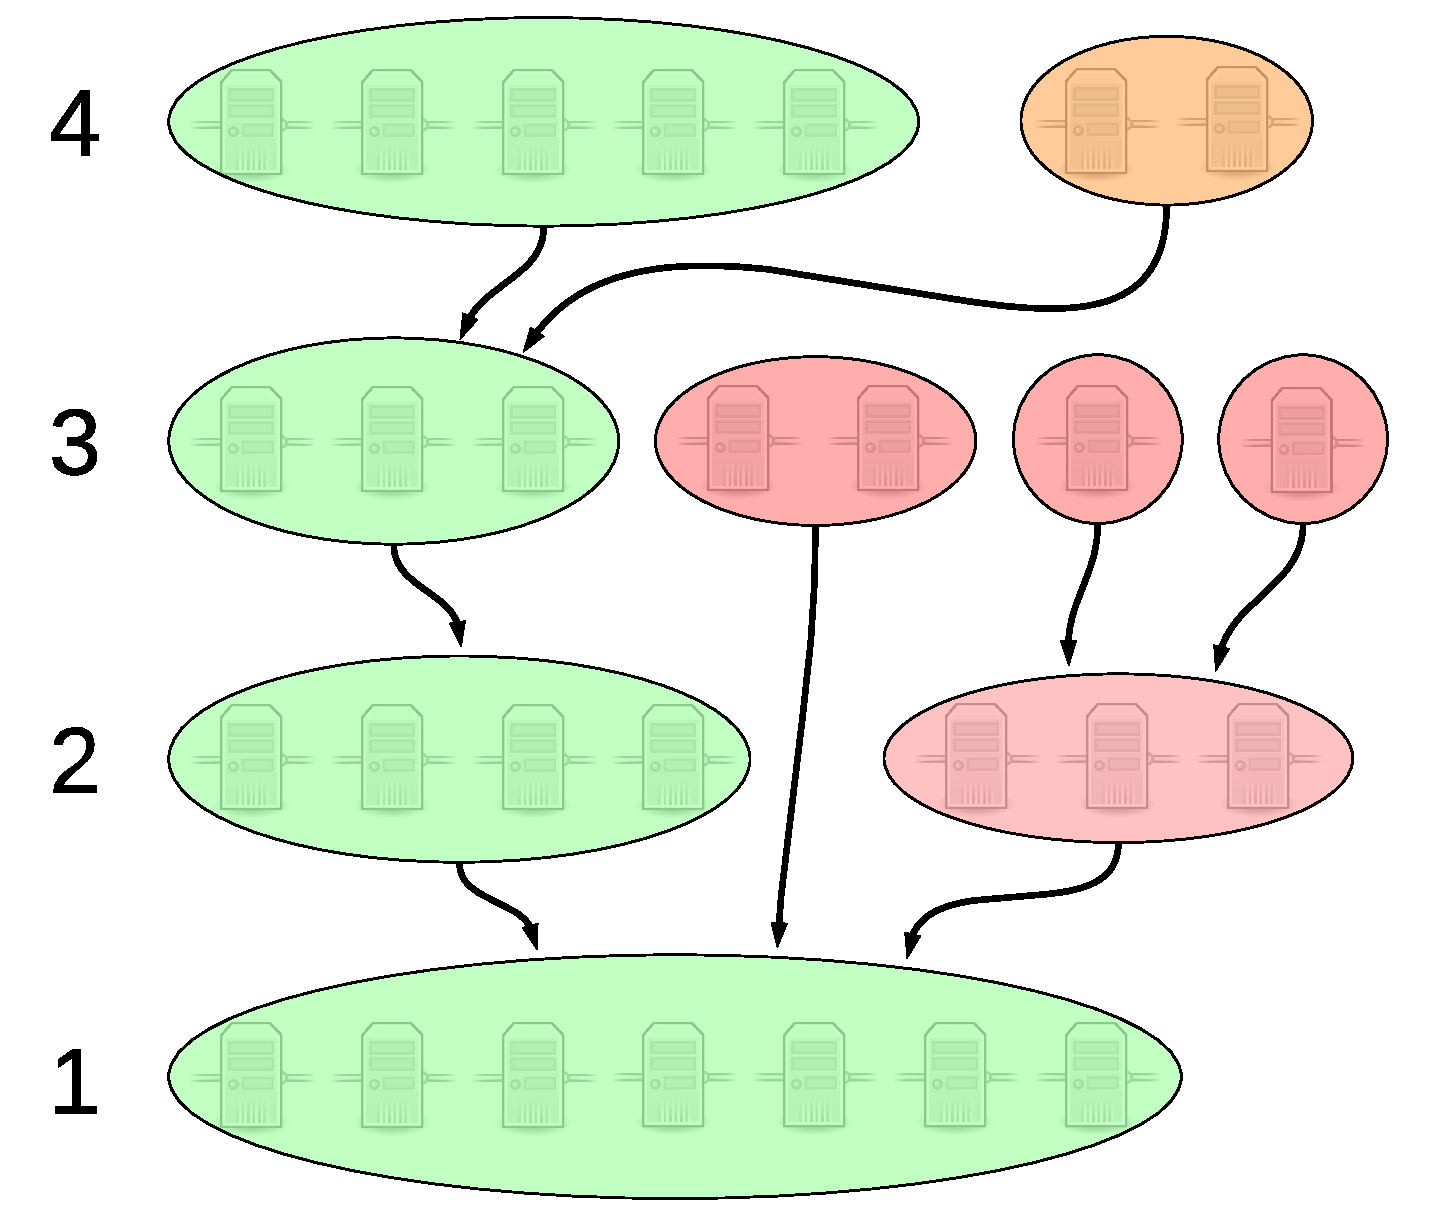
\includegraphics[width=0.4\linewidth]{../assets/images/LucidCharts/Page-chain2.pdf}
%	\caption{THIS IS A PLACEHOLDER IMAGE. TODO: create diagram of lottery-results timeline. The responsibilities of each Quorum are divided into two distinct parts: first, a lottery period where ``tickets'' are accepted and recorded; and second, a naming period where a fixed number of applicants receive names. The beginning of the Quorum and the lottery coincides with the publication of $ \mathcal{G}(t) $ in the consensus (Section \ref{sec:rngProcess}) while the beginning of the naming period corresponds to the appearance of $ \mathcal{G}(t) $ by the directory authorities.}
%	\label{fig:lotteryTimeline}
%\end{figure}

\subsubsection{Record Operations}
\label{sec:recordOps}

% todo: I'd like to remove PoW from records, but then how would clients verify that the work was done? Would they get the original ticket too?
% at the current or original PoW difficulty? How is this handled? -maybe unnecessary detail

OnioNS also supports common operations on names. Bob, an owner of an onion service, may construct modify, renew, transfer, or delete records and issue the records to the Quorum. In all cases, Bob sets the \emph{type} field to the appropriate record type. Once received, mirrors hold the record in a queue and apply them at 00:00 UTC each day by the protocol specified in Section \ref{sec:qQualification}. Thus updates take up to 24 hours to propegate through OnioNS.

Bob can modify his registration by changing \emph{secondaryAddrs}, \emph{subdomains} or \emph{contact} fields. Bob may also transfer the registration to a new owner by issuing a transfer record, which contains an additional field: \emph{recipientKey}, the public RSA key of the new onion service. This transfer request can be authenticated since Bob's record is signed, similar to a Bitcoin transaction. Bob may also relinquish control of his name by issuing a deletion record. Bob does not need to recompute proof-of-work for any of these records as these operations are cheap for the Quorum to apply. However, OnioNS names expire after 90 days, so name owners must periodically renew registrations to maintain ownership. This can be done by issuing a renew ticket with an updated $ \mathcal{G}(i) $ and recalculating the proof-of-work algorithm. The PoW requirement here reduces the risk of name squatting.

%todo: analysis: non-winners will likely try again. Won't this impact the PoW-difficulty adjustment?

\subsubsection{Domain Query}

Alice only needs Bob's ticket or his latest record to contact Bob by his meaningful name. She then uses the Merkle tree structure to verify that her name server responds with the correct ticket or record, or to achieve authenticated denial-of-existence if her query has no corresponding data structure. Let Alice type a domain $ d $ into the Tor Browser.

\begin{enumerate}
	\item Alice contacts a name server Charlie via his onion service.
	\item \label{step:ask} Alice asks Charlie for a ticket or record $ r $ containing $ d $.
	\item Charlie extracts the second-level name $ n $ from $ d $.
	\item If $ r $ exists, Charlie returns $ r $, the leaf node containing $ n $, and all the nodes from the leaf to the root and their sibling nodes.
	\item If $ r $ does not exist, Charlie returns two adjacent leaves $ a $ and $ b $ (and the nodes on their paths and siblings) such that $ a(\mathit{name}) < n < b(\mathit{name}) $, or in the boundary cases that $ a $ is undefined and $ b $ is the left-most leaf or $ b $ is undefined and $ a $ is the right-most leaf.
	\item Alice verifies the authenticity or non-existence of $ r $ by 
		\begin{enumerate}
			\item Asserting that $ n $ is either contained in the subtree or that $ n $ is spanned by the subtree leaves, respectively.
			\item Asserting the correctness of the hashes in the subtree.
			\item Asserting that the root hash matches the root hash published by the largest agreeing set of Quorum nodes, by validating every Quorum node's signature of its published root hash. %todo: does this last bit match database inheritance?
		\end{enumerate}
	\item If these assertions fail, Alice knows that Charlie is dishonest and she must repeat this protocol with a different mirror.
	\item If $ d $ in $ r $ points to a domain $ d_{2} $ which has a .tor pseudo-TLD, Alice jumps to \ref{step:ask} and queries for $ d_{2} $.
	\item Alice computes Bob's .onion address from $ r(\mathit{pubHSKey}) $ or randomly selects an .onion address from $ r(\mathit{secondaryAddrs}) $ (if present), proceeding in a round-robin fashion until she contacts Bob over the onion service protocol.
\end{enumerate}

It is impractical for Alice to download the whole database from all Quorum nodes over slow 6-hop onion service circuits. Alice uses the Merkle tree to verify the authenticity (or non-existence) and uniqueness of $ r $ with minimal networking costs even when the mirror Charlie is dishonest. This in turn requires trusting that the largest agreeing subset of the Quorum has published the correct root hash. We show in our security analysis that this assumption holds in most cases even if the Quorum is partially compromised.

Note that, although Alice needs to check all the Quorum nodes' signatures of the root hash, she does not need to do so for every Domain Query. Instead, this can be done once every registration period (24 hours) after which the records are updated. In this way, the signature verification cost is amortized.

%by synchronize against the OnioNS network and downloading the database from the Quorum, but this is impractical in most environments. Tor's median bandwidth for 6-hop onion circuits is approximately 188 KB/s (see Fig. \ref{fig:6HopBw}) so for the sake of convenience data transfer must be minimized. Therefore Alice can simply fetch minimal information and rely on her existing trust of members of the Tor network.

\subsubsection{Onion Query}

OnioNS also supports reverse-hostname lookups. In an Onion Query, Alice issues an onion service address \emph{addr} to Charlie and receives back all Records that have \emph{addr} as either the owner or as a destination in their \emph{subdomain}. Alice may obtain additional verification on the results by issuing Domain Queries on the source .tor domains. We do not anticipate Onion Queries to have significant practical value, but they complete the symmetry of lookups and allow OnioNS domain names to have Forward-Confirmed Reverse DNS matches. We suggest caching destination onion service addresses in a digital tree (trie) to accelerate this lookup; a trie turns the lookup from $ \mathcal{O}(n) $ to $ \mathcal{O}(1) $ while requiring $ \mathcal{O}(n) $ time and $ \mathcal{O}(n) $ space to pre-compute the cache.

% The idea here is that although everyone gets a proportionally-higher increase in PoW difficulty, it's acceptable by innocent parties (an extra 36 minutes is not that much) but the attacker now has to spend 48 hour of CPU (18 more hours) to get 30 tickets. If the attacker has a fixed budget for 30 hours of CPU time he'll be unable to make 30 tickets in lottery 3, but rather only 30/1.6=18. The difficulty never decreases, so if the number of tickets in the lottery is blinded from everyone except the Quorum, a point will be reached where the statistics are no longer in the attacker's favor, leading him to conclude that it's no longer worth it.

%\setlength{\belowcaptionskip}{-10pt}

% infrastructure (Authorative servers) (server management), registration process

\vspace{-5px}

\section{Security Analysis}
\label{sec:Analysis}

In this section, we analyze the security of the Onion Name System with regard to our security goals and  threat model. We supplement with a statistical analysis of the Quorum in Appendix \ref{sec:qSize} and \ref{sec:qRotation}.

\subsection{Global Randomness}
\label{sec:GlobalRand}

The beacon $ \mathcal{G}(t) $ should satisfy several security properties: unpredictable, unbiased, universally sampleable, and publicly verifiable \cite{BonneauCG15}. The latter two properties follow directly from the construction. The first two depends on the security of the Bitcoin blockchain. The unpredictability can be quantified by the (computational) min-entropy of the beacon, while the unbiased property is defined by the statistical closeness of $ \mathcal{G}(t) $ to an $m$-bit uniformly random string. In \cite{BonneauCG15}, the authors showed that this beacon generates 32 near-uniform random bits every 10 minutes. This would be sufficient for our system: if we assume $ \left\vert{Q}\right\vert = 127 $, then each Tor router is sampled at least  $\approx 2\%$ chance to be in a Quorum, which is much higher than $2^{-32}$.

The above assumes normal operation when honest parties control the majority of the computational power in the Bitcoin network. Next, we analyze the security of this assumption itself. Bitcoin miners, who perform the PoW, are rewarded with an agreed-upon bounty for generating a new block as well as the cumulation of transaction fees. These provide an incentive to solve the proof-of-work problem.  While miners originally attempted to solve the PoW problem independently, a community of miners may organize themselves into a ``mining pool''. Each miner in the pool attempts to find a solution to the PoW problem in the common block. When the PoW is solved, the reward is split across miners according to contributed processing power  \cite{eyal2015miner}. Since this is more financially rewarding, the vast majority of Bitcoin's hashrate is performed in this way. The top seven mining pools are shown in Fig. \ref{fig:poolHashrates}.

%While Bitcoin miners originally used CPUs for mining, in recent years miners have shifted to GPUs and then to specialized hardware such as FPGAs and ASICs which are more energy efficient and generally more financially viable.   (i.e. the rate of SHA-256 hashes, each a possible solution to the PoW)

%\renewcommand{\arraystretch}{1.1}
%\newcolumntype{L}[1]{>{\hsize=#1\hsize\raggedright\arraybackslash}X}%
%\newcolumntype{R}[1]{>{\hsize=#1\hsize\raggedleft\arraybackslash}X}%
%\newcolumntype{C}[2]{>{\hsize=#1\hsize\centering\arraybackslash}X}%
%\begin{table}[h]
%	\small
%	\vspace{-8px}
%	\centering
%	\begin{tabularx}{0.9\linewidth}{ | C{1} || C{1} || }
%    	%\textbf{Mining Pool} & \textbf{Percentage} \\ \hline
%    	F2Pool & 27\% \\ \hline
%		AntPool & 19\% \\ \hline
%		BTCC Pool & 15\% \\ \hline
%		BW.COM & 10\% \\ \hline
%		BitFury & 10\% \\ \hline
%		Kano CKPool & 4\% \\ \hline
%		Slush & 4\% \\ \hline
%		(All others) & 12\% \\ \hline
%  	\end{tabularx}
%  	\caption{Distribution of the top seven mining pools in the Bitcoin network as of June 2016 \cite{BitcoinHashrate}.}
% 	\label{fig:poolHashrates}
%  	\vspace{-24px}
%\end{table}

%\renewcommand{\arraystretch}{1.1}
\begin{table}[h]
	\small
	\vspace{-8px}
	\centering
	\begin{tabularx}{0.6\linewidth}{ | C{1} || C{1} || }
		%\textbf{Mining Pool} & \textbf{Percentage} \\ \hline
		F2Pool & 27\% \\ \hline
		AntPool & 19\% \\ \hline
		BTCC Pool & 15\% \\ \hline
		BW.COM & 10\% \\ \hline
		BitFury & 10\% \\ \hline
		Kano CKPool & 4\% \\ \hline
		Slush & 4\% \\ \hline
		(All others) & 12\% \\ \hline
	\end{tabularx}
	\caption{Distribution of the top seven mining pools in the Bitcoin network as of June 2016 \cite{BitcoinHashrate}.}
	\label{fig:poolHashrates}
	\vspace{-27px}
\end{table}



%\begin{figure}[htbp]
%	\vspace{-7px}
%	\centering
%	\includegraphics[width=0.7\linewidth]{../assets/analysis/bitcoin_hashrates.eps}
%	\caption{D}
%	\label{fig:poolHashrates}
%	\vspace{-10px}
%\end{figure}

As of June 2016, the aggregrate Bitcoin hashrate is 1.446 EH/s, or $ 1.446 \times 10^{18} $ hashes/second \cite{BitInfoCharts}. An attacker could compromise the security of the Bitcoin blockchain through a 51\% attack, wherein the attacker controls the majority of the hashrate and can thus control the longest chain. This can occur if either F2Pool, AntPool, and BTCC Pool collude (as they would then control 61\% of the hashrate) or if an attacker introduce more than 1.446 EH/s of computational power into the network. The most cost-effective and energy-efficient ASIC miners are capable of up to 4.7 TH/s, 0.25 watts/GH, and an initial up-front cost of \$520 USD \cite{MiningHwGuide}. Based on these figures, we estimate that a 51\% attack would cost \$158 million USD and would draw 395 megawatts. Therefore, so long as F2Pool, AntPool, and BTCC Pool do not collude, the honest majority computation power assumption in Bitcoin holds.

We also must analyze whether this beacon is resistant to manipulation attacks. In \cite{BonneauCG15}, the authors considered the scenerios where the attacker bribes the miners in order to suppress certain valid blocks and thus make the beacon predictable or otherwise favorable to the attacker.  They model a manipulation-resistant lottery scheme as a finite-state Markov process and found that the attacker must possess high stakes in the outcome of a lottery to be economically feasible. In this paper, we apply the same  methodology to analyze the security of the beacon. We can model the Quorum generation as a single-stage lottery where $|Q|$ nodes are chosen at a time using one beacon (i.e., $|Q|$ numbers derived from $ \mathcal{G}(t) $). The attacker controls the Quorum only if $Q$ contains the majority of malicious nodes. Thus, it has a binary reward function:
\begin{eqnarray}
A(s) = \left\{
\begin{array}{ll}
W \quad: \quad s\in S_*\\
0 \quad: \quad s\notin S_*
\end{array}
\right.
\end{eqnarray}
where $W$ is the reward of controlling the Quorum and $S_*$ is the state set of all Quorum node combinations where malicious nodes gain the majority. Denote $p$ the probability that attacker wins an unmanipulated lottery (the Quorum compromise probability, or the aggregated probability of states $S_*$), then $p$ is very small according to our analysis in Appendix \ref{sec:qSize}. For instance, when $|Q|=63$, percentage of colluding routers is 20\%, $p = 5.5\e{-16} $ (referring to Fig. \ref{fig:quorumWeightedMajority}). Thus, following Eq. (4) in \cite{BonneauCG15}, the attack is advantageous whenever $W>\frac{1}{p}$ Bitcoins. This amounts to  $\$4.3\e{17}$; suppose there are $50,000$ onion names in Tor as of now, each of them needs to worth \$8.6 trillion. This means it is practically infeasible for the attacker to bribe the miners to manipulate the beacon and Quorum generation in OnioNS. %While our beacon is also used for the domain registration lottery, similar analysis can be done to show the manipulation-resistance against the beacon for the registration lottery.

\subsection{Integrity Guarantees}
\label{sec:integrityG}

% They are an integral component in the ZFS file system, Bitcoin, Apache's Cassandra NoSQL database, \cite{CassandraDatabase} and in many other applications.
Merkle trees are widely used to achieve secure verification of very large data structures.  The security of the Merkle tree rests on the underlying hash function and its resistance to second pre-image attacks. During a Domain Query, clients fetch a subtree from mirrors, verify the integrity of the ticket or record against the leaf node, and recompute and verify the hashes of the subtree. The second pre-image attack resistance of SHA-256 prevents mirrors from forging or falsely claiming non-existence of a ticket or record. Clients also check the subtree value against the Quorum's published hashes, preventing mirrors from forging the subtree or returning an obsolete subtree. This approach provides strong integrity guarantees for both existent and non-existent records even if the mirror is malicious.

In the unlikely scenario that the attacker controls the majority of nodes in a Quorum,  the attacker can modify or substitute existing records during that Quorum's lifetime, which can mislead clients. However, a malicious Quorum cannot overwrite history (e.g. records from past Quorums) because the previous Quorums maintain a read-only copy of its own historical records. These historical records can also be stored by other mirrors, the current Quorum, or an external server. A client can send the same query to past Quorums to see if the records differ. If they do and the current Quorum does not provide explanatory proof (such as a modification or transfer record) then the client can detect expired/recaptured domains or malicious substitutions and should warn the user. We introduce a flag into our software for this purpose, which will also serve as a deterrent to malicious Quorums.

% Tor's directory authorities distribute consensus weight based on each router's computational and bandwidth capabilities relative to all other routers. 
Tor's resistance to Sybil attack helps to ensure the integrity of the Quorum and the security of OnioNS in general. New routers must demonstate long uptime and high reliability before they receive notable consensus weight. The arguably most prominent Sybil attack occured in December 2014 when members of the Lizard Squad group introduced approximately 3,300 new Tor routers. Although Lizard Squad then controlled more than half of the size of the Tor network, their routers collectively had 0.2743\% of the consensus weight. The Sybil attack was noticed by the Tor community and the offending routers were banned from the network. Small-scale Sybil attacks have also been detected through community-developed tools such as SybilHunter \cite{winter2016identifying}.

%\vspace{-20px}

\subsection{Lottery}
\label{sec:lotteryAnalysis}

%  in order to improve their chances of winning the lottery
Our lottery uses proof-of-work as a barrier-of-entry and awards names to a fixed number of onion services in any period to limit abuse. Here, we consider powerful adversaries with significant computational capabilities who may register many tickets as part of a land rush or to perform a denial-of-registration (DoR) attack. On the other hand, we anticipate that honest onion services will only attempt to register a single name, therefore they may be assumed to be computationally weak. We analyze our scheme's resilience against attacks in Section \ref{sec:lotteryAnalysisAppendix}. We found that with appropriate selection of the difficulty threshold, the attacker's expected number of winning names is approximately equal to the total number of winners scaled by the portion of its computation effort over the combined effort of attacker and all the legitimate registrants. Here, we recommend an initial value for the difficulty threshold, $ d_{\textit{th}} $. % and recommend design parameters for the lottery

Our analysis suggests that to effectively mitigate DoR attacks, we should set the difficulty level of innocent onion services to $ \frac{1}{4} $ of the expected maximum difficulty that a high-end CPU can obtain in 24 hours. This means that high-end CPUs should take about six hours to generate a lottery ticket. We benchmarked the performance of our reference implementation of the proof-of-work algorithm on low-end and high-end consumer-grade hardware. An Intel Core2 Quad Q9000 2.00 GHz Penryn CPU from late 2008 performed 1,773.7 PoW iterations per second on one CPU core and 6,165.9 i/s on all four CPU cores. Our high-end machine held an Intel i7-6700K 4.0 GHz Skylake CPU from 2015 and performed 8709.2 i/s on one CPU core and 33,930 i/s on eight cores. Since each iteration is independent probability event, the following formula derives the minimum value $ v_{\textit{th}} $ such that a CPU at $ S $ i/s has a 50\% chance to compute the result to the PoW in six hours:
\begin{equation}
v_{\textit{th}} \approx \frac{0.5 \cdot 2^{256}}{6 \cdot 60 \cdot 60 \cdot S}
\end{equation}
We consider that the i7-6700k represents the upper-end of consumer CPUs and use this formula to recommend $ v_{\textit{th}} = 2^{223.55} $ and $d_{\textit{th}} =256-224=32$ bits. Even with lower-end CPUs, fewer utilized cores, or a higher difficulty, the proof-of-work algorithm will generate a valid ticket eventually. We also suggest halving $ v_{\textit{th}} $ every two years so as to keep pace with a global average increase in computational power. With a sufficiently high value of lottery winners and a sufficiently low value for $ v_{\textit{th}} $, we believe that our lottery can resist a well-resourced adversary while simultaneously serving computationally-weak innocent parties.

%\renewcommand{\arraystretch}{1.3}
%\newcolumntype{L}[1]{>{\hsize=#1\hsize\raggedright\arraybackslash}X}%
%\newcolumntype{R}[1]{>{\hsize=#1\hsize\raggedleft\arraybackslash}X}%
%\newcolumntype{C}[2]{>{\hsize=#1\hsize\centering\arraybackslash}X}%
%\begin{table}[h]
%	\small
%	\begin{tabularx}{\linewidth}{ | C{1} || C{1} || C{1} || }
%    	\textbf{Description} & \textbf{$ M_{a} $ (ms)} & \textbf{$ M_{b} $ (ms)} \\ \hline
%    	Parsing JSON & 5.21 & 2.42 \\ \hline
%		$ \mathcal{H}(x) $ & 4.35 & 2.15 \\ \hline
%		$ V_{\mathit{RSA}}(m, E) $ & 6.35 & 2.74 \\ \hline
%		Total Time & 15.91 & 7.31 \\
%  	\end{tabularx}
%  	\caption{Client side time to verify a record (verifying the onion service's signature). }\label{tab:verifytime}
%\end{table}

%
%We consider that Craig that has access to efficient cloud computation, such as Amazon EC2. A compute-optimized instance, such as c4.large in California, costs appropriately 1 USD for 11 CPU core-hours on an Intel Xeon E5-2666 processor. In Table \ref{table:PoWtime}, we use \href{https://www.cpubenchmark.net/}{cpubenchmark.net} to convert this to the equivalent quantity of computation from a selection of Intel i7 CPUs, which are commonly found in high-end consumer-grade computers.

% , which will be accepted as long as $ \mathit{rand} $ is updated to the $ \mathcal{G}(i) $



%\begin{center}
%	\vspace{-5mm}
%	\begin{table}[htp]
%		\hspace{5 mm}
%  		\begin{tabular}{ | c | c | c | c | c | }
%  		\textbf{CPU} & \textbf{Speed} & \textbf{vCPUs} & \textbf{CPU Hours} & \textbf{Wall Time} \\ \hline
%  		c4.large & 24804 & 2 & 11 & 7.33 \\ \hline
%  		i7-5960X	 & 16002 & 16 & 17.05 & 1.42 \\ \hline
%  		i7-5930K & 13666 & 12 & 19.96 & 2.21 \\ \hline
%  		i7-4930K & 13074 & 12 & 20.87 & 2.32 \\ \hline
%  		i7-3930K & 12080 & 12 & 22.58 & 2.51 \\ \hline
%  		i7-4790K & 11228 & 8 & 24.30 & 4.05 \\ \hline
%  		i7-6700K & 11028 & 8 & 24.74 & 4.12 \\ \hline
%  		i7-4790 & 10034 & 8 & 27.19 & 4.53 \\ \hline
%  		i7-6700 & 9962 & 8 & 27.38 & 4.56 \\
%		\end{tabular}
%		\caption{The average time to complete the proof-of-work across various computational resources. These CPUs utilize hyper-threading; we assume that a single vCPU provides 75 percent of the power of a real core.}
%		\label{table:PoWtime}
%	\end{table}
%	\vspace{-10mm}
%\end{center}

%Selecting the number of winners in our lottery requires balancing the demand from innocent requests for names against the threat of en-mass registrations by adversaries. If the number of winners is too low, it is too difficult for innocent HS administrators to claim a name. On the other hand, too many winners allows computationally-powerful domain squatters to claim many names. Both scenarios negatively impact the usability of our system. While it is difficult to accurately predict honest demand for our system, we can estimate it by examining the number of popular onion services on the Tor network.

% As $ T_{i} $ is initially blinded, it is difficult for the adversary to determine in advance if this threshold is reached. This scheme also means that the system adapts in response to an increase in global average computational speed as the barrier-of-entry becomes too low.

\subsection{DNS Leakage}

Accidental leakage of .tor lookups over the Internet DNS via human mistakes or misconfigured software may compromise user privacy. This vulnerability is not limited to OnioNS and applies to any pseudo-TLD; Mohaisen and Thomas observed .onion lookups on root DNS servers at a frequency that corresponded to external global events and highlighting the human factor in those leakages \cite{thomasmeasuring}. Closing this leakage is difficult. Arguably the simplest approach is to introduce whitelists or blacklists into common web browsers to prevent known pseudo-TLDs from being queried over the Internet DNS. Such changes are outside the scope of this work, but we highlight the potential for this leak.

%We require no personally-identifiable information in domain registration and client queries are stateless and indistinguishable. We protect all communication into and inside OnioNS with Tor circuits, further enhancing user privacy. Our use of the Merkle tree provides strong integrity guarantees. The network as a 

%routers with high consensus weight must maintain high uptime, therefore we can assume that they all agree. This is also a good assumption since routers that are temporarily offline resynchronize when they come online again.

%Second, registrations are authenticable, which can be reduced to the security of the Merkle hash tree and to the assumption that the largest subset of Quorum nodes are honest. We verify this assumption in Section \ref{sec:QSelection} and \ref{sec:qSize}. Domain uniqueness also stems from the above assumption, relying on honesty of Quorum nodes to avoid collisions. Quorum selection is a random process assuming security of the commitment algorithm run by the directory authorities, which we analyse in Section \ref{sec:RandGeneration}. 

\vspace{-5px}

\section{Evaluation}
\label{sec:Evaluation}

\subsection{Implementation}

We have build a reference implementation of the Onion Name System in C++11 as a supplement to this work. We use JSON-RPC on top of microhttpd \cite{microhttpd} (a small HTTP server library) for networking and the Botan \cite{BotanLib} library for most cryptographic operations. We encode all the data structures in JSON and base64-encode binary data. Our code is licensed under the Modified BSD License, identical to Tor, and is available for Linux through a software repository at our onion service, \href{http://onions55e7yam27n.onion}{http://onions55e7yam27n.onion}. % JSON is significantly more compact than XML, but retains user readability and its support of basic primitive types is highly applicable to our needs. Since JSON is usually not capable of carrying binary values, we encode all non-ASCII values (such as SHA-256 hashes) in base64. 

\begin{figure}[t!]
	\centering
	\vspace{-8px}
	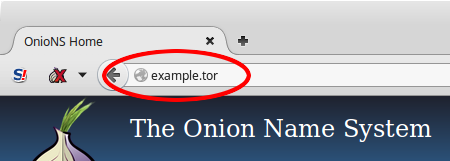
\includegraphics[width=0.85\linewidth]{../assets/images/example.png}
	\caption{We load our onionsite, available at \href{http://onions55e7yam27n.onion}{``onions55e7yam27n.onion''}, transparently under the ``example.tor'' domain. The OnioNS software launches with the Tor Browser.}
	\label{fig:prototypeExample}
	\vspace{-12pt}
\end{figure}

We divided our software into three parts: OnioNS-client, OnioNS-server, and OnioNS-HS, with OnioNS-common as a shared library dependency. OnioNS-client negotiates with the user's Tor software to MitM all requests for torified TCP streams. It filters for our .tor pseudo-TLD while allowing all other lookups (IPv4, .onion, or DNS) to pass unimpeded. Once it intercepts a request for a .tor domain, it performs a Domain Query and rewrites the domain to a .onion address before allowing Tor to bind the request to a circuit. This approach preserves backwards-compatibility, achieving a design objective and enhancing usability. The OnioNS-server simply binds to a localhost TCP port and performs our protocols. OnioNS-HS is a command-line utility that prompts the user for domain information, performs the proof-of-work, and uploads the ticket or record to the current Quorum. In all three cases, our software functions with minimal configuration. % Tor router administrators must then configure their Tor to host a onion service and bind it to the same localhost port so that OnioNS-server may be reached from the outside.

\subsection{Integration Test}

We have deployed a small testing network of Quorum and mirror servers. We first created an onion service for our project, set up a small web server, and used Shallot to generate a semi-meaningful address, \href{http://onions55e7yam27n.onion}{``onions55e7yam27n.onion''}. We then used OnioNS-HS to create a lottery ticket for ``example.tor'' and then to transmit it to the Quorum. This sole ticket won the lottery and we received our name. Our ticket then propagated through the network to mirrors. Finally, we installed our client software into Tor Browser 6.0.1, a fork of Firefox 45.2.0 ESR. We typed ``example.tor'' into the Tor Browser and the request was intercepted, resolved through a Domain Query, and rewritten to \href{http://onions55e7yam27n.onion}{``onions55e7yam27n.onion''}. The Tor binary then communicated with our onion service and returned the contents back to the Tor Browser. This process did not require any further user input and occurred behind-the-scenes, so the Tor Browser retained the ``example.tor'' name in the address bar and in the mouse-over text for relative hyperlinks. We illustrate the result in Fig. \ref{fig:prototypeExample}. The software performed asynchronously and allowed normal browsing to both the Internet and other onion services while it resolved ``example.tor''.


\subsection{Performance}

\subsubsection{Client-Side Overhead}

We measured the client-side overhead of record verification after a Domain Query. We tested the performance of our OnioNS-HS and OnioNS-client software on two machines, $ M_{a} $ and $ M_{b} $, the Q9000 and i7-6700k CPUs mentioned earlier. We measured the wall-time needed for a client to verify a record or ticket and averaged 200 samples. The results are shown in Table \ref{tab:verifytime}.

%\renewcommand{\arraystretch}{1.1}
%\newcolumntype{L}[1]{>{\hsize=#1\hsize\raggedright\arraybackslash}X}%
%\newcolumntype{R}[1]{>{\hsize=#1\hsize\raggedleft\arraybackslash}X}%
%\newcolumntype{C}[2]{>{\hsize=#1\hsize\centering\arraybackslash}X}%
%\begin{table}[h]
%	\small
%	\vspace{-8px}
%	\centering
%	\begin{tabularx}{0.9\linewidth}{ | C{1} || C{1} || C{1} || }
%    	\textbf{Description} & \textbf{$ M_{a} $ (ms)} & \textbf{$ M_{b} $ (ms)} \\ \hline
%    	Parsing JSON & 5.21 & 2.42 \\ \hline
%		$ \mathcal{H}(x) $ & 4.35 & 2.15 \\ \hline
%		$ V_{\mathit{RSA}}(m, S, E) $ & 6.35 & 2.74 \\ \hline
%		Total Time & 15.91 & 7.31 \\
%  	\end{tabularx}
%  	\caption{Client side time to verify a record (verifying the onion service's signature). }\label{tab:verifytime}
%  	\vspace{-24px}
%\end{table}


\renewcommand{\arraystretch}{1.0}
\begin{table}[h]
	\small
	\vspace{-8px}
	\centering
	\begin{tabularx}{0.85\linewidth}{ | C{1} || C{1} || C{1} || }
		Description & $ M_{a} $ (ms) & $ M_{b} $ (ms) \\ \hline
		Parsing JSON & 5.21 & 2.42 \\ \hline
		$ \mathcal{H}(x) $ & 4.35 & 2.15 \\ \hline
		$ V_{\mathit{RSA}}(m, S, E) $ & 6.35 & 2.74 \\ \hline
		Total Time & 15.91 & 7.31 \\
	\end{tabularx}
	\caption{The processing time required to verify a record. These measurements also apply to Quorum nodes and mirrors as they also verify tickets and records.}\label{tab:verifytime}
	\vspace{-24px}
\end{table}

The measurements show that clients can fully validate a record in less than 20 ms even on low-end hardware. Clients must also verify the Merkle tree proof from the mirror to authenticate record and confirm its uniqueness, and they must verify the router descriptors of all Quorum nodes in the consensus in order to authenticate the Merkle tree root hash. The overhead associated for Merkle tree verification is tree height ($ log_2(n) $) multiplied by the cost of $ \mathcal{H}(x) $. We can estimate the overhead of verifying router descriptors by multiplying the above numbers by $ \left\vert{Q}\right\vert $. For example, if $ \left\vert{Q}\right\vert = 127 $, then $ M_{b} $ takes $928$ ms. Note that this is a one-time cost per registration period.

% $ M_{b} $ outperformed $ M_{a} $ in all instances and we observed that single iteration of scrypt dominated the total validation time, matching our expectations. Obviously, higher-end CPUs can complete an iteration of scrypt in less time, but nevertheless the proof-of-work is the largest source of CPU cost for clients, mirrors, and Quorum nodes. Although we anticipate that this is an acceptable load on all parties, clients on extremely limited hardware may elect to skip the proof-of-work verification step at the cost of some security.

\subsubsection{Communication Overhead}
\label{sec:commOverhead}

Although Tor is a low-latency network, all OnioNS communications occur over six-hop onion service paths through Tor, which introduces latency into most of our protocols. The exact round-trip latency is highly dependent on queuing delays, processing latency, and the speed of each router selected by either party, as well as the length and speed of the links between the routers. The latency is most significant for clients and adds an additional delay between the time that a user enters an OnioNS domain into the Tor Browser and the moment that Tor begins loading the onion service. 

In May 2016 we conducted 10,000 measurements of the communication overhead of onion service paths through the Tor network. Each endpoint was hosted on a 24 Mbits AT\&T residential connection. Before each measurement, we cleared Tor's state file for both the client and the onion service, forcing both endpoints to generate fresh circuits and select new guard nodes. This allows our measurements to reflect the expected performance in a distributed environment wherein the clients and onion services select their own circuit. We then measured circuit construction to the onion service, the average time of three round trips, and the bandwidth measured during a transfer of a 2 MB payload. We observed that the median circuit construction overhead was 3952 ms, the median circuit latency is 470 ms, and the median bandwidth is 188 KB/s. We have provided supporting box plots of our results in Section \ref{sec:commOverheadAppendix}. % We also measured the circuit construction overhead associated with connecting to an onion service. 

We expect that a ticket or record would be less than 1 KiB. The mirror must transmit two SHA-256 hashes for each node in the Merkle tree to ensure verifiability. If OnioNS contains $ Z $ names, then the expected byte size of a serialized Merkle subtree is approximated by $ 2 \cdot (49 + e) \cdot \log_{2}(Z) $ where 49 is the byte size of a base64-encoded SHA-256 hash and $ e $ represents markup and other formatting overhead in the transmission and is approximately 98 in our implementation. Assuming 470 ms RTT and 188 KB/s median bandwidth, the client can download up to 99.6 KB of Merkle subtree data to stay within sub-second performance. The expected size of the subtree is 99.6 KB when $ Z = 2^{339} $, suggesting that the Domain Query scales to a very large number of names. The client can eliminate circuit construction overhead by connecting to a mirror at startup.


\subsubsection{Quorum Scalability}

In the Domain Registration protocol (section \ref{sec:ticketGeneration}) potential registrants upload tickets and records to all Quorum nodes. The committment form of these tickets must be uploaded within a short time period (e.g., five minutes) to minimize any information leakage to a potential attacker. Our analysis in Appendix \ref{sec:qSize} recommends $ \left\vert{Q}\right\vert = 127 $, so registrants must upload tickets to 127 Quorum nodes within this small window. Considering the aforementioned overhead of 6-hop circuits, in August 2016 we used the same setup as described above to measure the average time required to upload to a variable Quorum size. Our results, shown in Table \ref{table:uploadTime}, show that more than a minute is needed to upload to 127 Quorum nodes. Based on these measurements, we recommend a window of 5 minutes, which also provides a margin of error for clock skew.

\begin{table}[h]
	\small
	\vspace{-8px}
	\centering
	\begin{tabularx}{0.7\linewidth}{ | C{1} || C{1} || }
		Quorum Size & Avg. Time (sec) \\ \hline
		7 & 4.62 \\ \hline
		15 & 9.24 \\ \hline
		31 & 17.95 \\ \hline
		63 & 39.84 \\ \hline
		127 & 78.41 \\ \hline
		255 & 148.89 \\
	\end{tabularx}
	\caption{The time required to upload tickets to $ 2^{x}-1 $ Quorum nodes using 8 threads to accelerate communication.}
	\label{table:uploadTime}
	\vspace{-24px}
\end{table}

We also measured the storage, memory, and processing overhead for Domain Queries for a variable number of records. We generated fixed-size records of $ \approx $ 1 KB each with random names and followed Authenticated Denial-of-Existence algorithm to construct a Merkle tree. Since Table \ref{tab:verifytime} and Appendix \ref{sec:commOverheadAppendix} show that the overall time is dominated by the overhead and latency of 6-hop circuits, we removed the network component and measured performance while querying from the same machine. Our results are shown in Table \ref{table:queryPerformance}.

\begin{table}[h]
	\small
	\vspace{-8px}
	\centering
	\begin{tabularx}{0.9\linewidth}{ | C{1} || C{1} || C{1} || C{1} || }
		Records & Disk (MB) & RAM (MB) & CPU ($\upmu$s) \\ \hline
		$ 2^{14} $ & 18 & 19 & 7 \\ \hline
		$ 2^{15} $ & 36 & 21 & 32 \\ \hline
		$ 2^{16} $ & 71 & 25 & 145 \\ \hline
		$ 2^{17} $ & 142 & 31 & 257 \\ \hline
		$ 2^{18} $ & 284 & 42 & 634 \\ \hline
		$ 2^{19} $ & 568 & 63 & 1285 \\ \hline
		$ 2^{20} $ & 1137 & 108 & 2272 \\
	\end{tabularx}
	\caption{The server-side storage and memory costs to hold the records and the Merkle tree, respectively, and the processing overhead for a Domain Query. The measurements occurred on one thread of the $ M_{b} $ machine with -O3 compiler optimizations.}
	\label{table:queryPerformance}
	\vspace{-24px}
\end{table}

The table suggests that the processing time is very light and scales logarithmically with respect to the number of records. This time can be further improved through multi-threading as multiple Domain Queries can easily be performed in parallel. The memory and storage costs both scale linearly as expected, as the Merkle tree contains $ \mathcal{O}(n) $ nodes. These nodes are relatively cheap to store in RAM. The CPU cost to answer a query is very low, since the Merkle tree is pre-computed. 


% Domain Queries have low latency and the local cache can further reduce overhead, which is especially helpful if cached records are part of a chain of resolutions. 

% For small downloads, such as records and the Merkle subtree, the round-trip time will be dominated by the path latency. If the client builds the path on startup, we expect OnioNS lookups to add less than one second of latency in most cases. Our implementation provides a client-side cache, which helps to avoid redundant time-consuming queries to remote mirrors.


% We conducted additional tests of latency and bandwidth. We conducted a total of 128 measurements from $ M_{a} $ to $ M_{b} $ across 16 unique Tor circuits. The client took between 1.4 and 4.2 seconds (averaging 3.4 seconds) to construct an ephemeral path to our onion service with an average 0.565 seconds of round-trip latency after the path was established. We observed an average bandwidth of 141 kB/s for large downloads. 


%\subsubsection{Usability}
%
%OnioNS is lightweight for clients, is straightforward for onion service administrators to use, and is easy for Tor router administrators to support. Our client software integrates well into the Tor Browser and starts and stops with the Tor Browser environment. As shown in Fig. \ref{fig:prototypeExample}, OnioNS resolves and loads onion services under a meaningful name transparently without requiring any user interaction, similar to traditional DNS requests over Tor circuits. Domain Queries have low latency and the local cache can further reduce overhead, which is especially helpful if cached records are part of a chain of resolutions. 
%
%OnioNS-HS enables onion service administrators to claim a name and locally manage record information. The Ticket Generation protocol has minimal prompts: it asks the user for the main domain name, a list of subdomains and destinations, and an optional PGP key. It then loads the onion service private key, performs the proof-of-work algorithm, and automatically uploads the ticket to the Quorum. We released a beta test of our software to Tor developers and volunteers and received positive feedback on the simplicity of the registration process.
%
%We achieve another primary usability benefit by introducing an automatic naming system for Tor onion services: 

\section{Discussions}
\label{sec:Discussions}

In this section we further discuss and compare our work with related works. Our work shares several similarities with Namecoin and OnionDNS. The Domain Query protocol uses a Merkle tree to minimize networking costs, akin to the Simplified Payment Verification (SPV) scheme \cite{nakamoto2008bitcoin} for thin clients in Bitcoin. Our authenticated denial-of-existence algorithm is analagous to NSEC3 in DNSSEC. However, our system also provides some features and practical advantages that Namecoin, OnionDNS, and DNSSEC do not.

OnioNS has significantly less overhead than Namecoin: unlike an append-only blockchain, our database can be modified or deleted in-place and mirrors only remember records for non-expired names. Namecoin does not provide any rate-limiting on name registration and is thus vulnerable to land-rushes, denial-of-registration, and domain squatting attacks. This is evident by the severely skewed distribution of wealth in Namecoin; 43.7\% of all Namecoins are held by the richest 10 addresses and 90.5\% are held by the richest 1,000 addresses. By contrast, 5.3\% and 37.5\% of all Bitcoins are held by the richest 10 and 1,000 addresses, respectively. \cite{BitInfoCharts} Additionally, Namecoin does not provide any mechanisms for authenticated denial-of-existence. Clients must either trust the server or download the blockchain to confirm the claim. We also note that as of June 2016, Namecoin has a hashrate of 440 PH/s, 30.4\% of Bitcoin's hashrate  \cite{BitInfoCharts}. Since we use Bitcoin's blockchain as a beacon to generate $ \mathcal{G}(t) $, we consider OnioNS more resistant to computationally-powerful adversaries than Namecoin.

% As we mentioned in Section \ref{sec:RelatedWorks}, it is difficult for users to anonymously acquire Namecoins, which they need to save DNS information into the blockchain.

Hashed Authenticated Denial of Existence \cite{rfc5155} (NSEC3) is an extension for DNSSEC which authenticates NXDOMAIN responses by DNS servers. NSEC3 uses a sorted list of hashed names to prove non-existence; the client can quickly verify that no record exists between two names that canonically span the target. This mechanism also aims to avoid zone enumeration. In our work, we adapt this approach to also provide an authenticated denial-of-existence mechanism. OnioNS and Namecoin both allow full enumeration of all registered domains; however we do not consider this a significant threat to our system as registrations do not contain personal information. Both systems operate under weaker adversarial models than GNS, which assumes than an attacker may participant in any role, may infiltrate the network by large-scale Sybil attack, and is assumed to have more computational power than all honest participants combined. Neither Namecoin, OnioNS, nor Tor provide full defenses against such well-resourced adversaries. Tor onion services may become de-anonymized under GNS' adversarial model so we do not assume that our adversaries are that powerful.

We introduce the \emph{secondaryAddrs} field into the record data structure to achieve load-balancing at a name level, similar to the round-robin scheme in Internet DNS. We note that other tools exist for this purpose such as OnionBalance \cite{OnionBalance}, which uses specialized descriptors to distributes onion service requests across multiple backend Tor instances. We reduce the additional communication overhead by load-balancing requests at the name level. OnioNS also load-balance across its network because clients will query randomly-selected mirrors for tickets or records. If this selection is skewed by consensus weight, then the load will be distributed according to the capabilities of each mirror.

In OnioNS, users trust the Quorum, Tor directory authorities, and Bitcoin during a query. We consider these trustworthy due to Tor's resistance to Sybil attack (Section \ref{sec:integrityG}), the economic defenses in Bitcoin (Section \ref{sec:GlobalRand}), and the low likelihood of Quorum compromise (Appendix \ref{sec:qSize} and \ref{sec:qRotation}). As we described in Section \ref{sec:integrityG}, an OnioNS client can also query past Quorum nodes for additional verification. Transfer and modification records also allow the mirror to prove the authenticity of updates and the user can be warned if the record changes and this proof is not received during a query.

%Merkle tree is similar to SPV clients
%Auth denial is similar to NSEC3
%Lottery is similar to OnionDNS
%Why ours is better than Namecoin
%	similar threats
%	Namecoin is vulnerable to land-rushing and DoR, registrations are cheap
%	hard to register anonymously, short of mining which is expensive
%	3.6x less hashrate
%	does not provide auth denial-of-existence
%	we can modify the database in-place, so we have less overhead
%
%richest 10 addresses hold 43.66\% of all Namecoins while the richest 1,000 address hold and top 1,000 ri addresses hold 44\% of all Namecoins
%
%% todo: why can't we just use the hashing order for the Merkle leaves?
%
%In this section we further discuss and compare our work with related works. The Onion Name System and Namecoin both achieve all three properties of Zooko's Triangle and share some similarities, but the two systems have different threat models and distinct design objectives.
%
%Namecoin's security rests on two primary assumptions: that its network is resistant to Sybil attacks and that more than 50 percent of the network's computational power is at least semi-honest. An attacker that controls the majority of the computational power (a ``51\% attack'') or that has carried out a successful Sybil attack may then disrupt communications, corrupt the integrity of the blockchain, or can provide malicious responses to clients. Namecoin, like Bitcoin, also usually requires that clients download a complete copy of the blockchain. This introduces significant network, storage, and CPU costs which grow linearly to the age and popularity of the Namecoin network, preventing Namecoin from scaling to the general population. These costs can be largely avoided if the client uses a Namecoin-compatible DNS server or a Simplified Payment Verification \cite{nakamoto2008bitcoin} (SPV) scheme. These approaches are vulnerable to a variety of attacks if the name server is malicious and neither approach provides authenticated denial-of-existence.
%
%By contrast, OnioNS' central security assumption is that Tor circuits provide privacy. This assumption implies that the majority of the directory authorities remain semi-honest and that Tor network remains resistant to Sybil attack and traffic analysis. We rely on these assumptions for all aspects of our system. Thus, we can use existing Tor infrastructure instead of introducing a new network, as Namecoin does. Moreover, if an attacker can compromise Tor circuits or de-anonymize onion services, then a privacy-enhanced naming system no longer becomes necessary or relevant. Unlike Namecoin, we do not rely on assumptions of computational power; while Craig can negatively impact the ability for innocent onion services to get a name, he cannot affect the security of OnioNS or disrupt network communications. Our system remains secure as long as the Quorum remains uncompromised and we demonstrate in the appendix that a sufficiently-large Quorum is strongly resistant to a Sybil attack on the Tor network.

 %End-users should select their naming system carefully according to their threat model.

\section{Conclusions and Future Work}
\label{sec:Conclusion}

% Our system resists Sybil attack and land rushes from computationally-powerful adversaries.
We have presented the Onion Name System (OnioNS), a decentralized, secure, and privacy-enhanced alternative DNS that maps globally-unique and meaningful names to onion service addresses. OnioNS enables any onion service administrator to anonymously claim a human-readable name for their server and clients to query the system in a privacy-enhanced manner. We introduce mechanisms that let clients authenticate existent names and denial-of-existence claims with minimal overhead. We use Bitcoin as a cryptographically-secure beacon and utilize the existing and semi-trusted infrastructure of Tor. This significantly narrows our threat model to already well-understood attack surfaces and allows our system to be integrated into Tor with minimal effort. Our reference implementation shows the automatic resolution of domain names, which will allow scaling beyond human-maintained directories. This demonstrates that OnioNS can address the major usability issue that has been with Tor onion services since their introduction in 2002.

Following publication, we will expand our implementation and pursuit deploying it onto the Tor network. OnioNS introduces new software and a new .tor pseudo-TLD but requires no changes to the Tor executable. OnioNS is also forwards-compatible to changes in Tor circuits or the onion service protocol and requires only small modifications to become compatible to \cite{TorProp224}, the proposed next generation of Tor onion services.

%Additionally, our implementation currently only supports ASCII characters in domain names, so in future work we will explore implementing Punycode to provide support for international character sets. Unlike the Internet DNS, we will disallow digits zero and one (similar to base32 encoding) in order to reduce the threat of phishing attacks from spoofed domains with indistinguishable characters.

\section{Acknowledgments}

We would like to thank Roger Dingledine, George Kadianakis, Yawning Angel, Nick Mathewson, and other Tor developers and volunteers within the community for their technical support and commentary on our work. We thank the anonymous reviewers for their insightful comments and suggestions that helped to significantly improve the paper, and also thank Rob Jansen for shepherding our paper. This work was partially supported by NSF grants CNS-1111539, CNS-1314637, CNS-1520552, CNS-1218085, and ACI-1547428.

% https://en.wikibooks.org/wiki/LaTeX/Bibliography_Management#Bibliography_styles
\bibliographystyle{amsplain} 
\bibliography{citations}

\appendix
\vspace{-5pt}
\section{Appendix}

%In this section we statistically analyse the Tor network and provide recommendations for the size and rotation rate of the Quorum.

\subsection{Quorum Size}
\label{sec:qSize}

In Section \ref{sec:threatModel}, we assume that an attacker, Mallory, controls some fixed $ f_{E} $ fraction of routers on the Tor network. Quorum selection may be considered as an $ \left\vert{Q}\right\vert $-sized random sample taken from an $ \left\vert{T}\right\vert $-sized population without replacement, where the population contains $ \left\vert{T}\right\vert \cdot f_{E} $ entities that we assume are compromised and colluding. Then the probability that Mallory controls $ \left\vert{E}\right\vert $ Quorum nodes is given by the hypergeometric distribution, whose probability mass function is shown in Equation \ref{eq:hypergeoPMF}.
 Mallory controls the Quorum if either  $ \left\vert{E}\right\vert > \frac{\left\vert{Q}\right\vert}{2} $, or $ \left\vert{E}\right\vert < \frac{\left\vert{Q}\right\vert}{2} $ when the largest agreeing subset of legitimate Quorum nodes has size smaller than $ \left\vert{E}\right\vert$. 
 % $ > \frac{\left\vert{Q}\right\vert - \left\vert{E}\right\vert}{2} $ honest Quorum nodes disagree (publish different Merkle tree roots) or if. 
The latter scenario is difficult to model theoretically or in simulation, but the probability of the former can be calculated. If all Quorum nodes are selected with equal probability, then $ \mathrm{Pr}(\left\vert{E}\right\vert > \frac{\left\vert{Q}\right\vert}{2}) $ is given by the $p$-value of the hypergeometric test for over-representation, expressed in Equation \ref{eq:compromiseProb}.

% This statistical analysis assumes that OnioNS servers remained synchronized with the rest of the network; however we feel that this assumption is reasonable because the assignment of consensus weight is in part dependent on availability and furthermore that temporarily offline OnioNS servers resynchronize at startup. 

%As we skew Quorum selection by consensus weight, we must also consider Tor's distribution of consensus weight in our analysis and probability estimations.

%The probability that Mallory controls $ \left\vert{E}\right\vert $ Quorum nodes is given by the hypergeometric distribution, whose probability mass function is shown in Equation \ref{eq:hypergeoPMF}.

\begin{align}
	\mathrm{Pr}(\left\vert{E}\right\vert) &= \frac{\binom{\left\vert{T}\right\vert \cdot f_{E}}{\left\vert{E}\right\vert}\binom{\left\vert{T}\right\vert - \left\vert{T}\right\vert \cdot f_{E}}{\left\vert{Q}\right\vert - \left\vert{E}\right\vert}}{\binom{\left\vert{T}\right\vert}{\left\vert{Q}\right\vert}}
	\label{eq:hypergeoPMF}
	\\
	\mathrm{Pr}(\left\vert{E}\right\vert > \frac{\left\vert{Q}\right\vert}{2}) &= \displaystyle\sum_{i=\ceil{\frac{\left\vert{Q}\right\vert}{2}}}^{\left\vert{Q}\right\vert} \frac{\binom{\left\vert{T}\right\vert \cdot f_{E}}{i}\binom{\left\vert{T}\right\vert - \left\vert{T}\right\vert \cdot f_{E}}{\left\vert{Q}\right\vert - i}}{\binom{\left\vert{T}\right\vert}{\left\vert{Q}\right\vert}}
	\label{eq:compromiseProb}
\end{align}

Odd choices for $ \left\vert{Q}\right\vert $ prevents the network from splintering in the event that the Quorum is evenly split across two databases. We provide the statistical calculations of Equation \ref{eq:compromiseProb} for various Quorum sizes in Fig. \ref{fig:quorumUnweightedMajority}.




%If all Quorum Candidates have an equal probability of selection, then the probability that $ \left\vert{E}\right\vert > \frac{\left\vert{Q}\right\vert}{2} $ is given by the $p$-value of the hypergeometric test for over-representation, expressed in Equation \ref{eq:compromiseProb}. 
%
%We skew Quorum selection by consensus weight, In the next section we estimate the probability of Mallory controlling the Quorum under this weighted selection under Tor's distribution of consensus weight
%
% analyse Tor's distribution of consensus weight and the probability of Mallory controlling the Quorum under this weighted selection.
%
%We also assume that Tor's assignment of consensus weight provides a defence against Sybil attack and thus weight the se we also calcu
%
%The Quorum is rotated every $ \Delta q $ days, so we must consider the implications of selections for both $ \left\vert{Q}\right\vert $ and $ \Delta q $.

%In Section \ref{sec:threatModel}, we assume that an attacker, Mallory, controls some fixed $ f_{E} $ fraction of routers on the Tor network. Quorum selection may be considered as an $ \left\vert{Q}\right\vert $-sized random sample taken from an $ \left\vert{T}\right\vert $-sized population without replacement, where the population contains $ \left\vert{T}\right\vert \cdot f_{E} $ entities that we assume are compromised and colluding. If our selection includes $ \left\vert{E}\right\vert $ Mallory-controlled routers, then Mallory controls the Quorum if either $ > \frac{\left\vert{Q}\right\vert - \left\vert{E}\right\vert}{2} $ honest Quorum nodes disagree or if $ \left\vert{E}\right\vert > \frac{\left\vert{Q}\right\vert}{2} $. The former scenario is hard to model theoretically or in simulation, but the probability of the latter can be statistically calculated. The Quorum is rotated every $ \Delta q $ days, so we must consider the implications of selections for both $ \left\vert{Q}\right\vert $ and $ \Delta q $.

\begin{figure}[h]
	\centering
	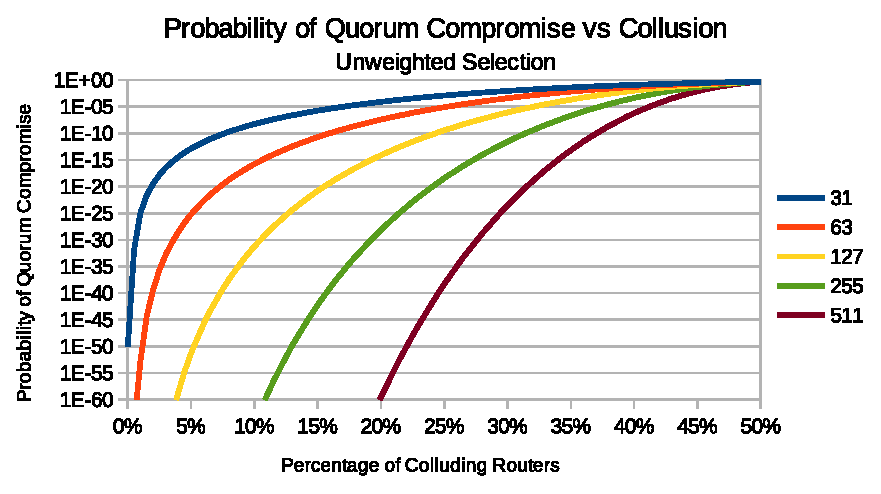
\includegraphics[width=\linewidth]{../assets/analysis/QuorumSelectionUnweighted.eps}
	\caption{The values for $ \mathrm{Pr}(\left\vert{E}\right\vert > \frac{\left\vert{Q}\right\vert}{2}) $ for Quorum sizes of 31, 63, 127, 255, and 511. All probabilities exceed 0.5 when more than 50 percent of the Tor network is under Mallory's control. We set our population to 4540 routers; the average number of routers with the Fast, Stable, and Running flags across all consensuses in June 2016 \cite{TorMetrics}.}
	\label{fig:quorumUnweightedMajority}
\end{figure}

However, we select Quorum members according to consensus weight, akin to router selection in a Tor circuit. The distribution of consensus weight (and thus the selection probabilities) for routers with the Fast, Stable, and Running flags closely follows an exponential distribution, as shown in Fig. \ref{fig:weightDist}. The figure suggests that the Tor network contains a low number of high-end routers and a large number of low-end routers.

\begin{figure}[h]
	\centering
	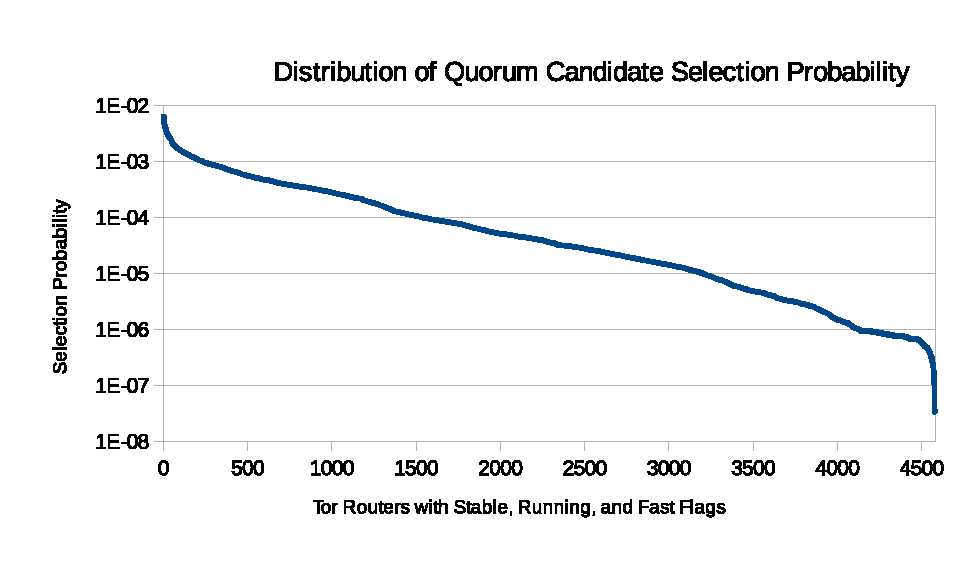
\includegraphics[width=\linewidth]{../assets/analysis/QuorumCandidateWeights.eps}
	\caption{The normalized distribution of consensus weights of Quorum candidates in June 2016, reflecting the probabilities of inclusion in the Quorum. The distribution may be modelled by an exponential trendline with $ R^{2} = 0.9884 $, but appears slightly super-exponential.}
	\label{fig:weightDist}
\end{figure}

We now re-examine Equation \ref{eq:compromiseProb} with regard to this distribution of consensus weight. Consider that the hypergeometric distribution describes the probability of selecting $ k $ Mallory-controlled routers in an $ \left\vert{Q}\right\vert $-sized Quorum from an $ N $-sized population containing $ K $ Mallory-controlled routers. Let $ L(x) $ be the probability distribution of selecting a router whose consensus weight is at the lowest $ x $ percentile. Then the probability of compromise is given by Equation \ref{eq:compromiseWeighted} where $ K $, the expected number of compromised routers in a population of size $ N $, is given by Equation \ref{eq:compromiseK}, and $ R $ is the probability that routers outside the  lowest $x$ percentile set are compromised.  Note that, the probability in Eq. \ref{eq:compromiseWeighted}  is an approximation of the actual probability of quorum compromise, as we model this problem as sampling balls from an urn without replacement, while the probability of choosing each ball is different. Currently there is no closed-form expression for such a problem. Thus we scale the number of compromised routers with their probabilities of being chosen.

We illustrate the probabilities against discrete values of $ x $ and various Quorum sizes in Fig. \ref{fig:quorumWeightedMajority} using $ N = 4540 $, consistent with the population in Fig. \ref{fig:quorumUnweightedMajority}.

\vspace{-5pt}
\begin{align}
	K &= N \cdot \left( \int_0^x(L(x)) + R \cdot \int_x^1(L(x)) \right)
	\label{eq:compromiseK}
	\\
	\mathrm{Pr}(\left\vert{E}\right\vert > \frac{\left\vert{Q}\right\vert}{2}) &= \displaystyle\sum_{i=\ceil{\frac{\left\vert{Q}\right\vert}{2}}}^{\left\vert{Q}\right\vert} \frac{\binom{K}{i}\binom{N - K}{\left\vert{Q}\right\vert - i}}{\binom{N}{\left\vert{Q}\right\vert}}
	\label{eq:compromiseWeighted}
\end{align}

In contrast to Fig. \ref{fig:quorumUnweightedMajority} which demonstrates that an unweighted selection leads to a high probability of compromise with small levels of collusion, Fig. \ref{fig:quorumWeightedMajority} suggests that biasing Quorum selection by consensus weight provides a strong defense against large-scale Sybil attacks. Indeed, even when 60 percent of the low-end Quorum candidates are malicious, most Quorum sizes produce negligible probabilities of compromise. We consider it reasonable to assume that low-end routers are under Mallory's control as these routers are the cheapest and logistically easiest to operate. Our approach remains resistant to this attack: these routers will be included in the Quorum very infrequently because of their low consensus weight.

\begin{figure}[h]
	\centering
	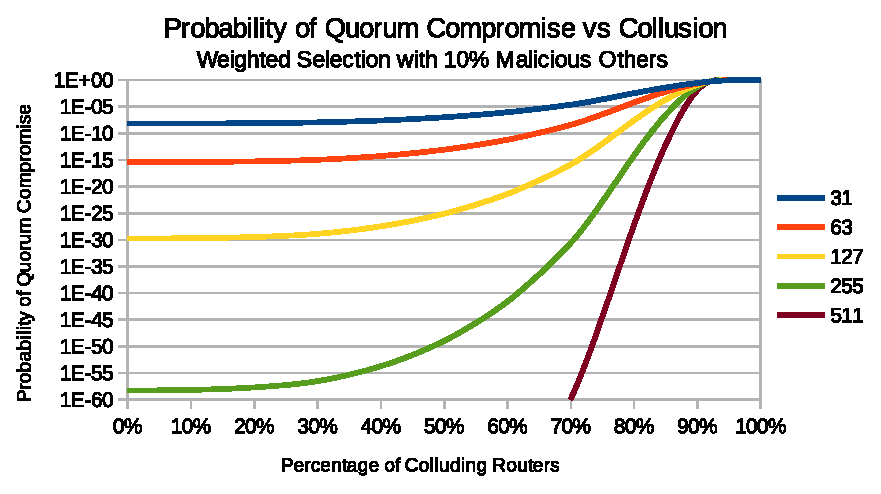
\includegraphics[width=\linewidth]{../assets/analysis/QuorumSelectionWeighted10.eps}
	\caption{The values for $ \mathrm{Pr}(\left\vert{E}\right\vert > \frac{\left\vert{Q}\right\vert}{2}) $ from Equation \ref{eq:compromiseWeighted} for various Quorum sizes. We assume that all routers $ \in L(x) $ are under Mallory's control, while routers $ \notin L(x) $ have a 10 percent chance of being under Mallory's control.}
	\label{fig:quorumWeightedMajority}
\end{figure}

Small Quorums are also more susceptible to node downtime or denial-of-service attacks. Fig. \ref{fig:quorumWeightedMajority} shows that the choices of $ \left\vert{Q}\right\vert = 31 $ is suboptimal; it is more easily compromised even with low levels of collusion. $ \left\vert{Q}\right\vert = 63 $ is more resistant, but not significantly more so. We therefore recommend $ \left\vert{Q}\right\vert \geq 127 $.

\subsection{Quorum Rotation}
\label{sec:qRotation}

In Section \ref{sec:threatModel}, we assume that $ f_{E} $ is fixed and does not increase in response to the inclusion of OnioNS on the Tor network. If we also assume that $ \left\vert{T}\right\vert $ is fixed, then we can examine the impact of choices for $ \Delta q $ and calculate the probability of Mallory compromising any Quorum over a period of time $ t $. Mallory's cumulative chances of compromising any Quorum is given by $ 1 - (1 - f_{c})^{\frac{t}{\Delta q}} $ where $ f_{c} $ is Mallory's chances of compromising a single Quorum. We estimate this over 10 years in Fig. \ref{fig:cumulativeProbability}.

\begin{figure}[h]
	\centering
	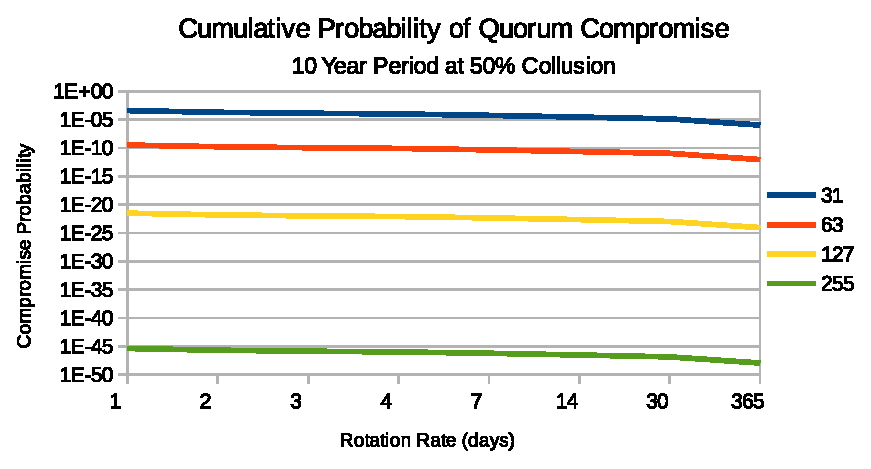
\includegraphics[width=\linewidth]{../assets/analysis/CumulativeMaliciousQuorumNew.eps}
	\caption{The cumulative probability that Mallory controls any Quorum at different rotation rates over 10 years at $ f_{E} = 50 $ for Quorum sizes 31, 63, 127, and 255. We base these statistics on the probabilities from Fig. \ref{fig:quorumWeightedMajority} at 50 percent collusion.}
	\label{fig:cumulativeProbability}
\end{figure}

%It also supports our earlier conclusion that the choices of $ \left\vert{Q}\right\vert = 31 $ and $ \left\vert{Q}\right\vert = 63 $ are suboptimal.
Fig. \ref{fig:cumulativeProbability} suggests that although larger values of $ \Delta q $ positively impact security, the choice of $ \left\vert{Q}\right\vert $ is more significant. Furthermore, even "stable" routers in the Tor network may be too unstable for very slow rotation rates, and small values for $ \Delta q $ also reduces the disruption timeline for a malicious Quorum. Therefore, based on Fig. \ref{fig:cumulativeProbability}, we further reiterate our recommendation of $ \left\vert{Q}\right\vert \geq 127 $ and suggest $ \Delta q = 7 $. Although a malicious Quorum would have the capabilities to deploy a variety of attacks on the network, the proper selections of $ \left\vert{Q}\right\vert $ and $ \Delta q $ reduces the likelihood of this occurring to near-zero probabilities. We consider this a stronger solution than introducing countermeasures to specific Quorum-level attacks.

\subsection{Lottery Analysis}
\label{sec:lotteryAnalysisAppendix}

As mentioned in Section \ref{sec:ticketGeneration}, the land-rush attacks are largely prevented by bootstrapping OnioNS with a reserved set of popular names, including existing Tor onion services. Second, we analyze the effectiveness of the lottery scheme, by studying the DoR attacker's best strategies and outcomes. Obviously, since there are many unpredictable factors in reality (e.g., the number of domain names honest services that will register every day, how everyone registers names, and each registrant's computation power), it is difficult to analyze against all possible scenarios. Thus, we make reasonable assumptions when necessary and try to abstract out the essential idea behind our lottery scheme.

\textbf{Notations and Assumptions}.
We assume there is a single well-resourced DoR attacker in the system, who controls $n_a>>1$ CPUs (or cores).  Each attacker CPU's speed is denoted as $s_a$. There are multiple ($m_g$) honest onion services which are homogeneous, i.e., each of them has $n_g=1$ CPU, with the same speed $s_g$, and only claims one name. The attacker may try to register $m_a\geq 1$ names.  Therefore, the total computation power of attacker is expressed in terms of CPU cycles: $P_a = s_a \cdot n_a$, while the total power of honest services is: $P_g=s_g \cdot m_g$. The ticket generation period is $\Delta t$. Assume that it takes $c_{\mathit{hash}}$ CPU cycles to do one SHA-256 operation and that the attacker equally spreads its computation power among $m_a$ names. For each of its claimed name, the maximum number of hash operations for the PoW that attacker can carry out during $\Delta t$ is: $\omega_a = \frac{P_a\cdot\Delta t}{m_a\cdot c_{\mathit{hash}}}$. Let the minimum PoW value $v_{\mathit{min}}$ he can compute during $\Delta t$ be equal to $\omega_a$ \footnote{This is an approximation. To obtain a value less than $v$, the expected number of hash operations is $2^{\mathit{256}}/v$.}, which is used as each of his ticket's weight  in the lottery. Similarly, for each honest onion service's ticket, we have $\omega_g = s_g\cdot\Delta t/c_{\mathit{hash}}$. The minimum difficulty every ticket needs to satisfy is denoted as $d_{\mathit{th}}$.

\textbf{Theoretical Analysis}.
Now we consider two extreme cases. First, there are no collisions among attacker's claimed names and honest services' names. Second, that there are a maximum number of collisions possible among those names. We assume that honest service's names are all unique and there can be at most two tickets per name under collision (one from attacker and one from honest service). In the first case, since the attacker's and honest services' tickets generally have different weights and probabilities of being chosen, the lottery process can be modeled as a random sampling process without replacement (urn model) with bias. This can be captured by the Wallenius' noncentral hypergeometric distribution: if an urn contains $m_a$ red balls (attacker's tickets) and $m_g$ white balls (honest services' tickets), totalling $N = m_a + m_g$ balls. Each red ball has the weight $\omega_a$ and each white ball has the weight $\omega_g$. The odds ratio is $\omega = \omega_a / \omega_g$. Then, $W\leq N$ balls (winners) are randomly sampled from this urn. Thus, the expected number of attacker's tickets chosen as winner is given by the positive solution $\mu$ to the following equation \cite{Wallenius}:

\begin{equation}
\frac{\mu}{m_a}+(1-\frac{W-\mu}{m_g})^\omega = 1 \label{eq-odds}
\end{equation}

Since the above equation does not have closed-form solution, we can solve it using numerical methods. 

In the second case, when the number of attacker's tickets  is smaller than honest services' ($m_a<m_g$),  each attacker's ticket has a collision with an honest service's ticket. For those collided names ($m_a$), no matter whose ticket is chosen, the other ticket is removed from the lottery. The rest of $m_g-m_a$ have no collisions. Thus, if we regard two  tickets under each collided name as a whole red ball, the non-collided tickets as white balls, this is again mapped to a Wallenius' noncentral hypergeometric distribution, with odds ratio being $\omega = (\omega_a+\omega_g) / \omega_g$, $m_a'=m_a$, $m_g'=m_g-m_a$.  Now the expected attacker winners is computed as: 
\begin{equation}
\mu'=\mu\cdot \frac{\omega_a}{ \omega_a+\omega_g},
\end{equation}
where $\mu$ is the solution to Eq. \ref{eq-odds}, with $m_a'$ and $m_g'$ as the parameters in it.

When the number of attacker's tickets is larger than honest services' ($m_a>m_g$), each honest service's ticket has a collision with an attacker's ticket. Similarly, we can derive the expected attacker winners in this sub-case:

\begin{equation}
\mu'=\mu+(W-\mu)\cdot \frac{\omega_a}{ \omega_a+\omega_g},
\end{equation}
where $\mu$ is again the solution to Eq. \ref{eq-odds}, with $m_a'=m_a-m_g$,  $m_g'=m_g$, and $\omega = \omega_a / (\omega_a+\omega_g)$ as the parameters in it. 

Finally, because of the minimum threshold difficulty requirement for every ticket's PoW, if $\omega_a<d_{\mathit{th}}$, that is, if $m_a>\frac{P_a\cdot \Delta t}{d_{\mathit{th}}\cdot c_{\mathit{hash}}}$, all of attacker's tickets will be removed and he will have zero winners in the lottery. 

\textbf{Numerical Results.} We did a numerical simulation in Matlab with the following parameter settings as an example. We assume $W=m_g=50$ (there are 50 honest onion services that win unique names each day), $s_g=s_a=3$ GHz, the total number of CPUs possessed by the attacker $n_a\geq 1$, $\Delta t=86400 s$ (one day), and $c_{hash}=512$ CPU cycles to do one SHA-256 operation (according to the benchmark results\footnote{https://www.cryptopp.com/benchmarks.html}). Also,  attacker's strategy $m_a$ is a variable, which can range from 1 to 1000. We plot the result as the expected number of attacker won tickets v.s. $m_a$, for both cases (with or without collisions), with different amount of attacker computation powers $n_a$. It can be seen from Fig. \ref{fig:lottery} that,  the attacker's expected winner size grows with $m_a$ and has a cutoff when its difficulty is less than the threshold. The blue dashed line stands for the power ratio, which is the fraction of the attacker's total computation power to the total power of attacker and honest services'. When  $m_a$ is larger than $n_a$ (the point when each of attacker's name is backed by equal computation power to a honest one), the  expected attacker winners grow at a decreasing rate, until the cutoff point. If we choose the threshold difficulty level to be a little smaller  than what legitimate service's computation power allows  (i.e., $1/4$ of the maximum difficulty level a legitimate high-end CPU can compute in a 24 hour period, shown in Fig. \ref{fig:lottery}), the maximum expected percentage of attacker's presence in the lottery winners  is approximately  the power ratio. This is important since the attacker needs to compete with the entire set of honest services' computation power to launch the DoR attack. The honest services always have a chance of being selected as winners regardless of the strength of the attacker.

Another observation is that in the name collision case when $m_a$ is small, the expected attacker winners is smaller than the no-collision case, but when $m_a$ is big, it is larger. This is because, when $m_a$ is small, honest onion services also have a chance being selected. Whenever that happens, it removes one ticket from the attacker, thus it reduces the chance of the attacker winning. 

Comparing with OnionDNS's domain registration method \cite{scaife2015oniondns}, if the attacker can estimate the number of honest services and their difficulty levels, in OnionDNS the attacker would win many names using the minimum difficulty level since most of them may not have a competitor, and if attacker has a higher difficulty level it wins an individual game deterministically. However, in our design, this is not possible due to the randomization and rate-limiting factor of the lottery, and also the fact that the lottery weight of a ticket is proportional to  their computation power dedicated to each ticket, which diminishes exponentially with the difficulty level of the PoW in each ticket. So it is not possible for an attacker gain overwhelming presence in the final set of winners. We consider that the registration schemes in OnionDNS and our work can potentially be complimentary since our lottery scheme is more suitable for a distributed Quorum.

\begin{figure}[t!]
	\centering
	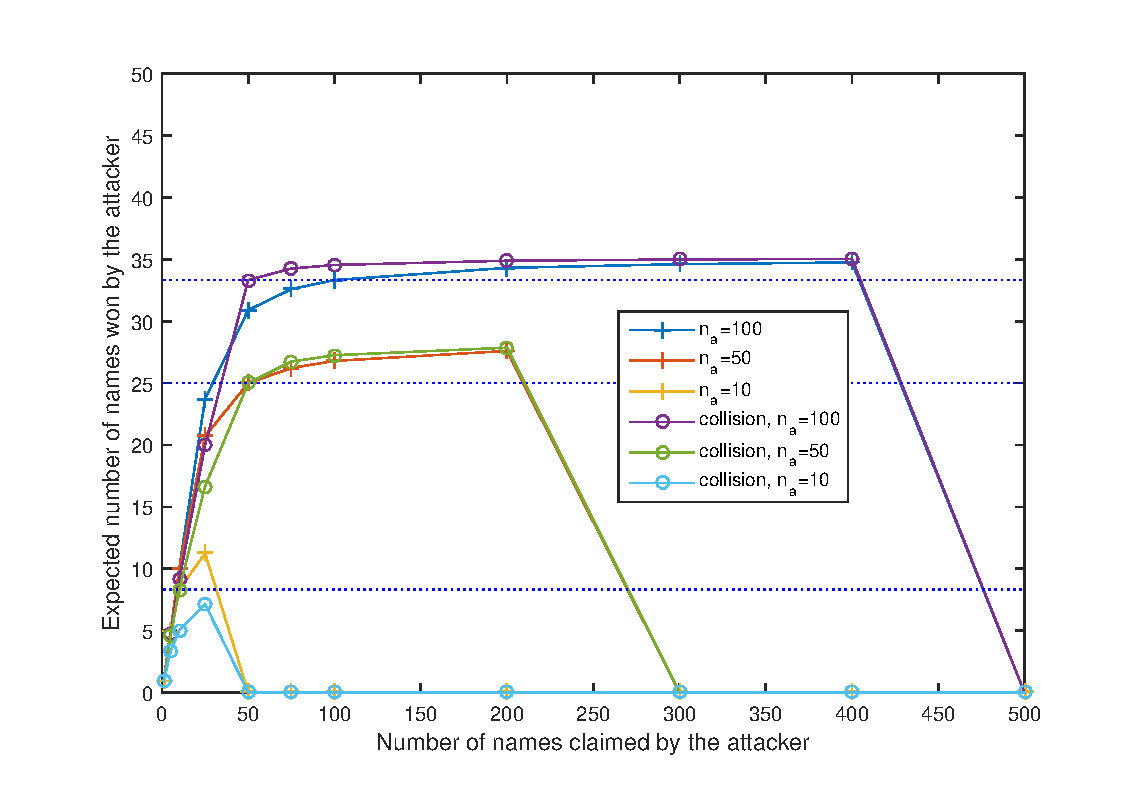
\includegraphics[width=\linewidth]{../assets/images/winners-allcases.eps}
	\caption{The expected number of attacker-won tickets in the lottery.}
	\label{fig:lottery}
	\vspace{-10pt}
\end{figure}

\newpage

\subsection{Communication Overhead of Onion Service Circuits}
\label{sec:commOverheadAppendix}

%\textbf{JV 3/13: To save space, I made this section and moved the box plots into it.}

As we mentioned in Section \ref{sec:commOverhead}, we measured the performance of 6-hop onion service circuits. We measured the time required to construct initial circuits to the onion service, the average round-trip time (RTT), and the bandwidth for a 2 MB payload. We performed 10,000 samples and reset Tor's state file on both endpoints each time, forcing each Tor instance to negotiate fresh circuits through the network. We provide box-and-whisker plots of our results in Fig. \ref{fig:6HopSetup}, \ref{fig:6HopLatency}, and \ref{fig:6HopBw}.

\begin{figure}[h]
	\centering
	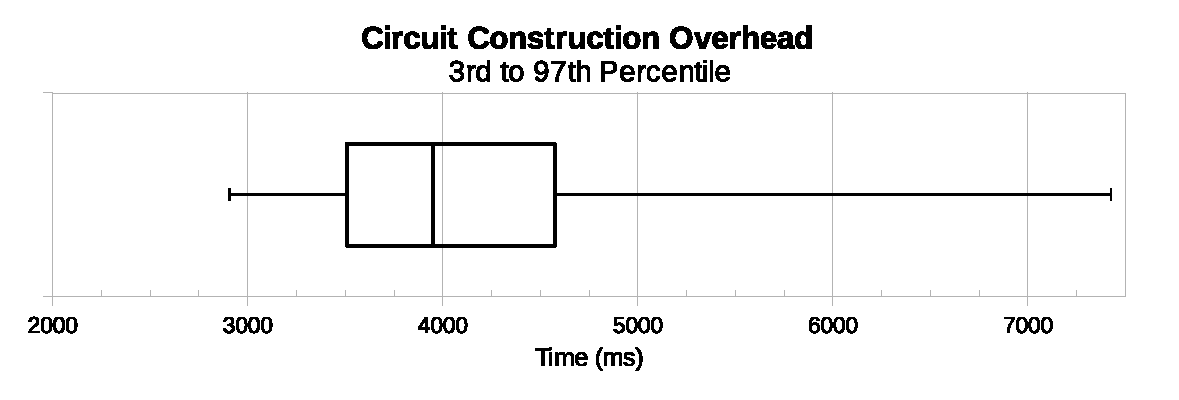
\includegraphics[width=\linewidth]{../assets/images/Tor/perf/circuit_construction_overhead.eps}
	\caption{The median overhead for connecting with an onion service is 3952 ms with a standard deviation of 1794 ms. The whiskers span the 3rd to 97th percentile at 2907 ms and 7353 ms, respectively.}
	\label{fig:6HopSetup}
	\vspace{10px}
	
	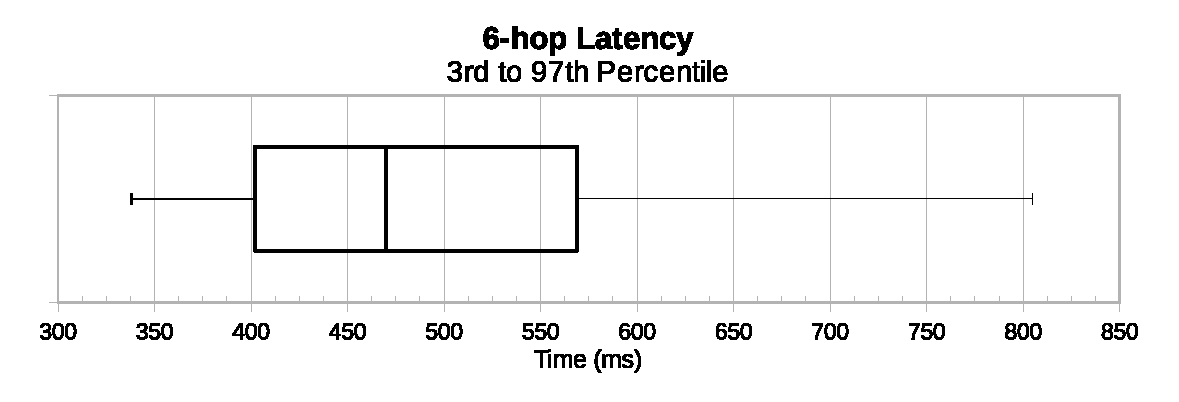
\includegraphics[width=\linewidth]{../assets/images/Tor/perf/6_hop_latency.eps}
	\caption{The median latency of an onion service circuit is 470 ms with a standard deviation of 184 ms. The 3rd and 97th percentile are 338 ms and 805 ms, respectively.}
	\label{fig:6HopLatency}
	\vspace{10px}
	
	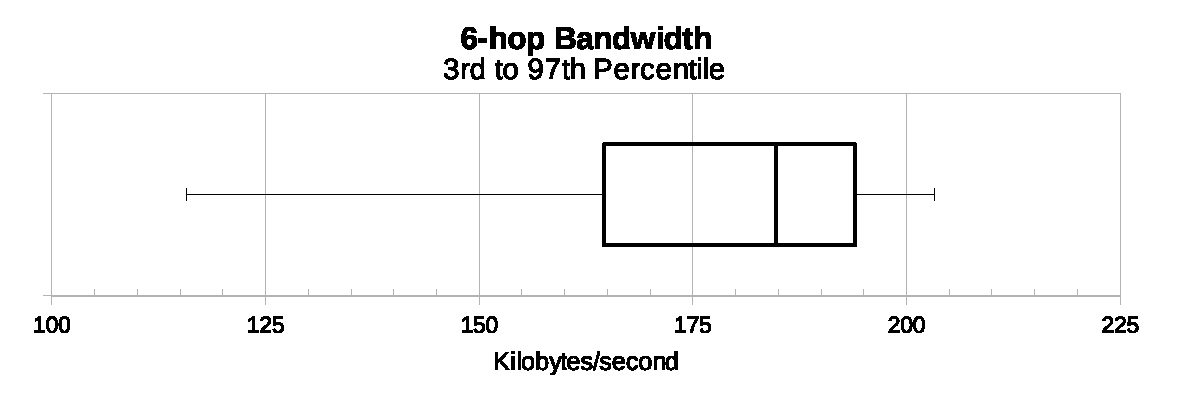
\includegraphics[width=\linewidth]{../assets/images/Tor/perf/6_hop_bw.eps}
	\caption{The median bandwidth for a 2 MB transfer over an onion service circuit is 188 KB/s with a standard deviation of 23 KB/s. The 3rd and 97th percentile are 116 KB/s and 203 KB/s, respectively.}
	\label{fig:6HopBw}
	\vspace{10px}
\end{figure}

%remove the following:
%\subsection{Derivation of Lottery Analysis Equations}
%
%In this section we derive and further clarify the lottery analysis equations that we introduced in Section \ref{sec:lottery}. We set the proof-of-work threshold, $ t_{d} $ according to
%\[
%	t_{d} = \frac{d_{b}}{\ceil{\frac{j}{\nWinners}}}
%\]
%
%Thus $ t_{d} = d_{b} $ for the first $ \nWinners $ tickets, $ t_{d} = \frac{d_{b}}{2} $ for the second set of $ \nWinners $ tickets, and so on. The sum of the coefficient is given by the $ n $th triangular number.
%\[
%	t(n) = \binom{n + 1}{2} = \frac{n \cdot (n + 1)}{2}
%\]
%
%We can then compute $ T(p) $ by deriving Equation \ref{eq:nTickets}.
%\begin{align*}
%	p &= d_{b} \cdot \nWinners \cdot (\frac{n \cdot  (n+1)}{2}) \\
%	\frac{p}{d_{b} \cdot \nWinners} &= \frac{n^{2} + n}{2} \\
%	0 &= n^{2} + n - \frac{2 \cdot p}{d_{b} \cdot \nWinners} \\
%	n &=  \frac{-1 + \sqrt{1 - 4(\frac{-2 \cdot p}{d_{b} \cdot \nWinners} - 2)}}{2} \\
%	n &= \frac{-1+ \sqrt{1 + \frac{8 \cdot p}{d_{b} \cdot \nWinners}}}{2} \\
%	T(p) &= \frac{\nWinners \cdot \sqrt{1 + \frac{8 \cdot p}{d_{b} \cdot \nWinners}} - \nWinners}{2}
%\end{align*}
%
%
%%In the scenario in Section \ref{sec:lottery}, Craig submits his tickets after $ \nWinners $ innocent actors. Thus Craig starts with $ t_{d} = 2 d_{b} $ and each must perform $ d_{b} \cdot \nWinners $ amount of work for each set in the base case.
%%\begin{align*}
%%	C_{w} &= d_{b} \cdot \nWinners \cdot (\frac{n \cdot  (n+1)}{2} - 1) \\
%%	C_{w} &= \frac{d_{b} \cdot \nWinners \cdot n \cdot  (n+1)}{2} - d_{b} \cdot \nWinners
%%\end{align*}
%%
%%This is Equation \ref{eq:nCraigTickets}. We can then solve for $ n $. %, the number of tickets that Craig can compute with $ C_{w} $ work.
%%\begin{align*}
%%	C_{w} &= d_{b} \cdot \nWinners \cdot (\frac{n \cdot  (n+1)}{2} - 1) \\
%%	\frac{C_{w}}{d_{b} \cdot \nWinners} &= \frac{n^{2} + n}{2} - 1 \\
%%	\frac{C_{w}}{d_{b} \cdot \nWinners} + 1 &= \frac{n^{2} + n}{2} \\
%%	\frac{2 \cdot C_{w}}{d_{b} \cdot \nWinners} + 2 &= n^{2} + n \\
%%	0 &= n^{2} + n - \frac{2 \cdot C_{w}}{d_{b} \cdot \nWinners} - 2 \\
%%	n &= \frac{-1 + \sqrt{1 - 4(\frac{-2 \cdot C_{w}}{d_{b} \cdot \nWinners} - 2)}}{2} \\
%%	n &= \frac{-1 + \sqrt{9 + \frac{8 \cdot C_{w}}{d_{b} \cdot \nWinners}}}{2}
%%\end{align*}
%%
%%\newpage
%%
%%We must then account for the fact that $ \nWinners $ tickets have already been submitted. This produces 
%%\begin{align*}
%%	n &= \frac{-1 + \sqrt{9 + \frac{8 \cdot C_{w}}{d_{b} \cdot \nWinners}}}{2} - 1 \\
%%	n &= \frac{-3 + \sqrt{9 + \frac{8 \cdot C_{w}}{d_{b} \cdot \nWinners}}}{2}
%%\end{align*}
%%
%%We then multiply by the size of each set, $ \nWinners $, resulting in Equation \ref{eq:nCraigTickets}.
%%\begin{align*}
%%	C_{t} = \frac{-3 \cdot \nWinners + \nWinners \sqrt{9 + \frac{8 \cdot C_{w}}{d_{b} \cdot \nWinners}}}{2}
%%\end{align*}
%%
%%The expected number of winning innocent onion services is the number of winners multiplied by the probability of selecting innocent onion services.
%%\begin{align*}
%%	\left\vert{W_{i}(\mathrm{innocent})}\right\vert &= \frac{\nWinners \cdot \nWinners}{\nWinners + C_{t}} \\
%%	\left\vert{W_{i}(\mathrm{innocent})}\right\vert &= \frac{\nWinners^{2}}{\nWinners + \frac{-3 \cdot \nWinners + \nWinners \sqrt{9 + \frac{8 \cdot C_{w}}{d_{b} \cdot \nWinners}}}{2}} \\
%%	\left\vert{W_{i}(\mathrm{innocent})}\right\vert &= \frac{2 \cdot \nWinners^{2}}{-\nWinners + \nWinners \cdot \sqrt{9 + \frac{8 \cdot C_{w}}{d_{b} \cdot \nWinners}}} \\
%%	\left\vert{W_{i}(\mathrm{innocent})}\right\vert &= \frac{2 \nWinners}{-1 + \sqrt{9 + \frac{8 \cdot C_{w}}{d_{b} \cdot \nWinners}}}
%%\end{align*}
%%
%%This is Equation \ref{eq:expInnocentWinners}. $ \left\vert{W_{i}(\mathrm{innocent})}\right\vert > 0 $ when $ \nWinners \geq 1 $, so Craig cannot prevent innocent onion services from claiming names. However, if $ C_{t} $ is sufficiently large, then $ \left\vert{W_{i}(\mathrm{innocent})}\right\vert < 1 $. If Craig can compute $ C_{R} $ amount of work, then we can express $ \left\vert{W_{i}(\mathrm{innocent})}\right\vert = 1 $ as
%%\[
%%	1 = \frac{2 \nWinners}{-1 + \sqrt{9 + \frac{8 \cdot C_{R}}{d_{b} \cdot \nWinners}}}
%%\]
%%
%%The inverse is Equation \ref{eq:resistance2DoR}, which computes the minimum amount of work required for Craig to carry out a denial-of-registration attack.
%%\[
%%	C_{R} = \frac{d_{b} \cdot \nWinners^{3} + d_{b} \cdot \nWinners^{2}}{2} - d_{b} \cdot \nWinners
%%\]
%


% that's all folks
\end{document}

